% Options for packages loaded elsewhere
\PassOptionsToPackage{unicode}{hyperref}
\PassOptionsToPackage{hyphens}{url}
\PassOptionsToPackage{dvipsnames,svgnames,x11names}{xcolor}
%
\documentclass[
  letterpaper,
]{scrbook}

\usepackage{amsmath,amssymb}
\usepackage{iftex}
\ifPDFTeX
  \usepackage[T1]{fontenc}
  \usepackage[utf8]{inputenc}
  \usepackage{textcomp} % provide euro and other symbols
\else % if luatex or xetex
  \usepackage{unicode-math}
  \defaultfontfeatures{Scale=MatchLowercase}
  \defaultfontfeatures[\rmfamily]{Ligatures=TeX,Scale=1}
\fi
\usepackage[]{kpfonts}
\ifPDFTeX\else  
    % xetex/luatex font selection
  \setmonofont[]{FiraMono}
\fi
% Use upquote if available, for straight quotes in verbatim environments
\IfFileExists{upquote.sty}{\usepackage{upquote}}{}
\IfFileExists{microtype.sty}{% use microtype if available
  \usepackage[]{microtype}
  \UseMicrotypeSet[protrusion]{basicmath} % disable protrusion for tt fonts
}{}
\makeatletter
\@ifundefined{KOMAClassName}{% if non-KOMA class
  \IfFileExists{parskip.sty}{%
    \usepackage{parskip}
  }{% else
    \setlength{\parindent}{0pt}
    \setlength{\parskip}{6pt plus 2pt minus 1pt}}
}{% if KOMA class
  \KOMAoptions{parskip=half}}
\makeatother
\usepackage{xcolor}
\setlength{\emergencystretch}{3em} % prevent overfull lines
\setcounter{secnumdepth}{5}
% Make \paragraph and \subparagraph free-standing
\ifx\paragraph\undefined\else
  \let\oldparagraph\paragraph
  \renewcommand{\paragraph}[1]{\oldparagraph{#1}\mbox{}}
\fi
\ifx\subparagraph\undefined\else
  \let\oldsubparagraph\subparagraph
  \renewcommand{\subparagraph}[1]{\oldsubparagraph{#1}\mbox{}}
\fi

\usepackage{color}
\usepackage{fancyvrb}
\newcommand{\VerbBar}{|}
\newcommand{\VERB}{\Verb[commandchars=\\\{\}]}
\DefineVerbatimEnvironment{Highlighting}{Verbatim}{commandchars=\\\{\}}
% Add ',fontsize=\small' for more characters per line
\usepackage{framed}
\definecolor{shadecolor}{RGB}{241,243,245}
\newenvironment{Shaded}{\begin{snugshade}}{\end{snugshade}}
\newcommand{\AlertTok}[1]{\textcolor[rgb]{0.68,0.00,0.00}{#1}}
\newcommand{\AnnotationTok}[1]{\textcolor[rgb]{0.37,0.37,0.37}{#1}}
\newcommand{\AttributeTok}[1]{\textcolor[rgb]{0.40,0.45,0.13}{#1}}
\newcommand{\BaseNTok}[1]{\textcolor[rgb]{0.68,0.00,0.00}{#1}}
\newcommand{\BuiltInTok}[1]{\textcolor[rgb]{0.00,0.23,0.31}{#1}}
\newcommand{\CharTok}[1]{\textcolor[rgb]{0.13,0.47,0.30}{#1}}
\newcommand{\CommentTok}[1]{\textcolor[rgb]{0.37,0.37,0.37}{#1}}
\newcommand{\CommentVarTok}[1]{\textcolor[rgb]{0.37,0.37,0.37}{\textit{#1}}}
\newcommand{\ConstantTok}[1]{\textcolor[rgb]{0.56,0.35,0.01}{#1}}
\newcommand{\ControlFlowTok}[1]{\textcolor[rgb]{0.00,0.23,0.31}{\textbf{#1}}}
\newcommand{\DataTypeTok}[1]{\textcolor[rgb]{0.68,0.00,0.00}{#1}}
\newcommand{\DecValTok}[1]{\textcolor[rgb]{0.68,0.00,0.00}{#1}}
\newcommand{\DocumentationTok}[1]{\textcolor[rgb]{0.37,0.37,0.37}{\textit{#1}}}
\newcommand{\ErrorTok}[1]{\textcolor[rgb]{0.68,0.00,0.00}{#1}}
\newcommand{\ExtensionTok}[1]{\textcolor[rgb]{0.00,0.23,0.31}{#1}}
\newcommand{\FloatTok}[1]{\textcolor[rgb]{0.68,0.00,0.00}{#1}}
\newcommand{\FunctionTok}[1]{\textcolor[rgb]{0.28,0.35,0.67}{#1}}
\newcommand{\ImportTok}[1]{\textcolor[rgb]{0.00,0.46,0.62}{#1}}
\newcommand{\InformationTok}[1]{\textcolor[rgb]{0.37,0.37,0.37}{#1}}
\newcommand{\KeywordTok}[1]{\textcolor[rgb]{0.00,0.23,0.31}{\textbf{#1}}}
\newcommand{\NormalTok}[1]{\textcolor[rgb]{0.00,0.23,0.31}{#1}}
\newcommand{\OperatorTok}[1]{\textcolor[rgb]{0.37,0.37,0.37}{#1}}
\newcommand{\OtherTok}[1]{\textcolor[rgb]{0.00,0.23,0.31}{#1}}
\newcommand{\PreprocessorTok}[1]{\textcolor[rgb]{0.68,0.00,0.00}{#1}}
\newcommand{\RegionMarkerTok}[1]{\textcolor[rgb]{0.00,0.23,0.31}{#1}}
\newcommand{\SpecialCharTok}[1]{\textcolor[rgb]{0.37,0.37,0.37}{#1}}
\newcommand{\SpecialStringTok}[1]{\textcolor[rgb]{0.13,0.47,0.30}{#1}}
\newcommand{\StringTok}[1]{\textcolor[rgb]{0.13,0.47,0.30}{#1}}
\newcommand{\VariableTok}[1]{\textcolor[rgb]{0.07,0.07,0.07}{#1}}
\newcommand{\VerbatimStringTok}[1]{\textcolor[rgb]{0.13,0.47,0.30}{#1}}
\newcommand{\WarningTok}[1]{\textcolor[rgb]{0.37,0.37,0.37}{\textit{#1}}}

\providecommand{\tightlist}{%
  \setlength{\itemsep}{0pt}\setlength{\parskip}{0pt}}\usepackage{longtable,booktabs,array}
\usepackage{calc} % for calculating minipage widths
% Correct order of tables after \paragraph or \subparagraph
\usepackage{etoolbox}
\makeatletter
\patchcmd\longtable{\par}{\if@noskipsec\mbox{}\fi\par}{}{}
\makeatother
% Allow footnotes in longtable head/foot
\IfFileExists{footnotehyper.sty}{\usepackage{footnotehyper}}{\usepackage{footnote}}
\makesavenoteenv{longtable}
\usepackage{graphicx}
\makeatletter
\def\maxwidth{\ifdim\Gin@nat@width>\linewidth\linewidth\else\Gin@nat@width\fi}
\def\maxheight{\ifdim\Gin@nat@height>\textheight\textheight\else\Gin@nat@height\fi}
\makeatother
% Scale images if necessary, so that they will not overflow the page
% margins by default, and it is still possible to overwrite the defaults
% using explicit options in \includegraphics[width, height, ...]{}
\setkeys{Gin}{width=\maxwidth,height=\maxheight,keepaspectratio}
% Set default figure placement to htbp
\makeatletter
\def\fps@figure{htbp}
\makeatother

% using text input is not working
% _quarto.yml

\usepackage{hyperref}
\usepackage{fancyvrb,newverbs,xcolor}
\usepackage{FiraMono} 
\usepackage{tikz}
\usepackage{xcolor}
\usepackage{soul}
%\usepackage[margin=0.5in]{geometry}
%\usepackage{afterpage}

\usepackage{geometry}
 \geometry{
 letterpaper,
bottom=0.8in,
top=0.8in,
left=0.8in,
right=0.8in,
includefoot
 }

%fontsize=9pt
% \geometry{
% paperwidth=6in,
% paperheight=9in,
% bottom=0.8in,
% top=0.8in,
% left=0.8in,
% right=0.8in
% }

%\setlength{\parskip}{0pt}
%
%\usepackage[compact]{titlesec}
%\titlespacing{\section}{0pt}{2ex}{1ex}
%\titlespacing{\subsection}{0pt}{1ex}{0ex}
%\titlespacing{\subsubsection}{0pt}{0.5ex}{0ex}
\makeatletter
\@ifpackageloaded{tcolorbox}{}{\usepackage[skins,breakable]{tcolorbox}}
\@ifpackageloaded{fontawesome5}{}{\usepackage{fontawesome5}}
\definecolor{quarto-callout-color}{HTML}{909090}
\definecolor{quarto-callout-note-color}{HTML}{0758E5}
\definecolor{quarto-callout-important-color}{HTML}{CC1914}
\definecolor{quarto-callout-warning-color}{HTML}{EB9113}
\definecolor{quarto-callout-tip-color}{HTML}{00A047}
\definecolor{quarto-callout-caution-color}{HTML}{FC5300}
\definecolor{quarto-callout-color-frame}{HTML}{acacac}
\definecolor{quarto-callout-note-color-frame}{HTML}{4582ec}
\definecolor{quarto-callout-important-color-frame}{HTML}{d9534f}
\definecolor{quarto-callout-warning-color-frame}{HTML}{f0ad4e}
\definecolor{quarto-callout-tip-color-frame}{HTML}{02b875}
\definecolor{quarto-callout-caution-color-frame}{HTML}{fd7e14}
\makeatother
\makeatletter
\@ifpackageloaded{bookmark}{}{\usepackage{bookmark}}
\makeatother
\makeatletter
\@ifpackageloaded{caption}{}{\usepackage{caption}}
\AtBeginDocument{%
\ifdefined\contentsname
  \renewcommand*\contentsname{Table of contents}
\else
  \newcommand\contentsname{Table of contents}
\fi
\ifdefined\listfigurename
  \renewcommand*\listfigurename{List of Figures}
\else
  \newcommand\listfigurename{List of Figures}
\fi
\ifdefined\listtablename
  \renewcommand*\listtablename{List of Tables}
\else
  \newcommand\listtablename{List of Tables}
\fi
\ifdefined\figurename
  \renewcommand*\figurename{Figure}
\else
  \newcommand\figurename{Figure}
\fi
\ifdefined\tablename
  \renewcommand*\tablename{Table}
\else
  \newcommand\tablename{Table}
\fi
}
\@ifpackageloaded{float}{}{\usepackage{float}}
\floatstyle{ruled}
\@ifundefined{c@chapter}{\newfloat{codelisting}{h}{lop}}{\newfloat{codelisting}{h}{lop}[chapter]}
\floatname{codelisting}{Listing}
\newcommand*\listoflistings{\listof{codelisting}{List of Listings}}
\makeatother
\makeatletter
\makeatother
\makeatletter
\@ifpackageloaded{caption}{}{\usepackage{caption}}
\@ifpackageloaded{subcaption}{}{\usepackage{subcaption}}
\makeatother
\makeatletter
\@ifpackageloaded{tcolorbox}{}{\usepackage[skins,breakable]{tcolorbox}}
\makeatother
\makeatletter
\@ifundefined{shadecolor}{\definecolor{shadecolor}{rgb}{.97, .97, .97}}{}
\makeatother
\makeatletter
\@ifundefined{codebgcolor}{\definecolor{codebgcolor}{HTML}{D3D3D3}}{}
\makeatother
\makeatletter
\ifdefined\Shaded\renewenvironment{Shaded}{\begin{tcolorbox}[frame hidden, boxrule=0pt, colback={codebgcolor}, enhanced, sharp corners, breakable]}{\end{tcolorbox}}\fi
\makeatother
\ifLuaTeX
  \usepackage{selnolig}  % disable illegal ligatures
\fi
\usepackage{bookmark}

\IfFileExists{xurl.sty}{\usepackage{xurl}}{} % add URL line breaks if available
\urlstyle{same} % disable monospaced font for URLs
\hypersetup{
  pdftitle={Data Science for Crime Analysis with Python},
  pdfauthor={Andrew P. Wheeler},
  colorlinks=true,
  linkcolor={Maroon},
  filecolor={Maroon},
  citecolor={Blue},
  urlcolor={Blue},
  pdfcreator={LaTeX via pandoc}}

\title{Data Science for Crime Analysis with Python}
\author{Andrew P. Wheeler}
\date{2025-10-07}

\begin{document}
\frontmatter
\maketitle

Data Science for Crime Analysis with Python

\copyright Andrew P. Wheeler 2024

ISBN 979-8-9903770-0-4 (ebook), ISBN 979-8-9903770-1-1 (paperback)

All rights reserved. No part of this publication may be produced or transmitted in any
form or by any means without prior written permission, with the exception of small excerpts for review. 
For permission contact Andrew P. Wheeler at andrew.wheeler@crimede-coder.com.

You can see my other work at \url{https://crimede-coder.com/}

\begin{tikzpicture}[scale=0.05]
\node[xshift=-1.5in,yshift=-1.5in]{
\includegraphics{chap_images/WLineRec.PNG}};
\end{tikzpicture}

% macros file to define verbatim environment
% which is the output of code samples
% https://tex.stackexchange.com/a/141128/8217

%\usepackage{fancyvrb,newverbs,xcolor}
%\usepackage{soul}

%\definecolor{cverbbg}{gray}{0.93}
\definecolor{cverbbg}{HTML}{ADD8E6}

\renewenvironment{verbatim}
 {\SaveVerbatim{cverb}}
 {\endSaveVerbatim
  \flushleft\fboxrule=0pt\fboxsep=.5em
  \colorbox{cverbbg}{%
    \makebox[\dimexpr\linewidth-2\fboxsep][l]{\BUseVerbatim{cverb}}%
  }
  \endflushleft
}

% https://gist.github.com/wusunlab/9c85fcb7472308a474e7c3fb443639ee
\definecolor{inlineBG}{HTML}{D3D3D3}
\sethlcolor{inlineBG}
\let\OldTexttt\texttt
\renewcommand{\texttt}[1]{\sethlcolor{inlineBG}{\ttfamily\hl{\mbox{#1}}}}

% https://tex.stackexchange.com/a/86702/8217
% to draw tikz in background

%https://tex.stackexchange.com/questions/70547/how-can-i-renew-includegraphics-to-always-use-shadowbox

\raggedbottom

\renewcommand*\contentsname{Table of Contents}
{
\hypersetup{linkcolor=}
\setcounter{tocdepth}{1}
\tableofcontents
}
\mainmatter
\bookmarksetup{startatroot}

\chapter*{Prefacio}\label{prefacio}
\addcontentsline{toc}{chapter}{Prefacio}

\markboth{Prefacio}{Prefacio}

Python es un lenguaje de programación de código abierto y gratuito. Te
permite escribir programas sencillos (o complejos) para que tu
computadora realice tareas. Como breve ejemplo, aquí tienes un fragmento
de código de Python que te indica la diferencia en el número de días
entre dos fechas. Las líneas que empiezan con \texttt{\#} son
comentarios en Python; las otras líneas realizan distintas operaciones
en código de Python. El texto en la parte gris de abajo es el código de
Python, y el texto de la sección azul es la salida del programa.

\begin{Shaded}
\begin{Highlighting}[]
\CommentTok{\# importing library to calculate times}
\ImportTok{from}\NormalTok{ datetime }\ImportTok{import}\NormalTok{ datetime}

\CommentTok{\# creating two datetime objects}
\NormalTok{begin }\OperatorTok{=}\NormalTok{ datetime(}\DecValTok{2022}\NormalTok{,}\DecValTok{1}\NormalTok{,}\DecValTok{16}\NormalTok{)}
\NormalTok{end }\OperatorTok{=}\NormalTok{ datetime(}\DecValTok{2023}\NormalTok{,}\DecValTok{1}\NormalTok{,}\DecValTok{16}\NormalTok{)}

\CommentTok{\# calculating the difference}
\NormalTok{dif }\OperatorTok{=}\NormalTok{ end }\OperatorTok{{-}}\NormalTok{ begin}

\CommentTok{\# printing the result}
\BuiltInTok{print}\NormalTok{(dif.days)}
\end{Highlighting}
\end{Shaded}

\begin{verbatim}
365
\end{verbatim}

Así que este es un programa trivial: podrías calcular el número de días
entre las dos fechas usando varias herramientas. El poder de saber
programar en Python es que puedes escribir código para realizar (casi)
cualquier cálculo que quieras. Un ejemplo común para un analista
criminal puede ser consultar una base de datos y crear una tabla de
conteos de delitos acumulados en lo que va del año para este año frente
al anterior. Luego puedes ejecutar el código cuando quieras, y este
actualizará las estadísticas acumuladas en lo que va del año con la
frecuencia que desees. En la práctica, un informe así no es más que
encadenar pequeños ejemplos de código como los de arriba en series de
operaciones más complejas.

\section*{¿Para quién es este libro?}\label{para-quiuxe9n-es-este-libro}
\addcontentsline{toc}{section}{¿Para quién es este libro?}

\markright{¿Para quién es este libro?}

Este libro está dirigido a personas sin experiencia (o con experiencia
inicial) en programación, pero que están interesadas en usar código para
realizar análisis cuantitativos y automatizar tareas. El público
principal al que va dirigido el libro está compuesto por analistas
delictivos, pero cualquier persona que busque iniciarse en la
programación y el análisis de datos debería encontrar útil el contenido
del libro. Además de los analistas delictivos, quienes deseen avanzar en
su carrera en un rol de ciencia de datos o realizar investigación a
nivel de posgrado (y que tengan formación en justicia penal) encontrarán
útil el libro y sus ejemplos.

Hay muchos recursos actuales sobre el uso de python en internet -- se
puede usar un motor de búsqueda para encontrar diversos recursos
completamente gratuitos en línea. Habitualmente escribo sobre
computación técnica en
\href{https://andrewpwheeler.com/}{andrewpwheeler.com}, que es gratuito
para que cualquiera lo lea. Sin embargo, estos recursos gratuitos a
menudo son desordenados y resultan muy difíciles para que los
principiantes los entiendan y se pongan en marcha. Cosas como ``¿Cómo
ejecuto un script sencillo de python?'' o ``¿Cómo instalo una biblioteca
de python?'' no son temas típicos que se cubran ni siquiera en
materiales introductorios de python en línea. Este libro pretende
constituir un recurso único para que las personas dedicadas al análisis
delictivo puedan empezar.

Mi intención con este libro no es solo presentar ejemplos de código en
python, sino también describir otros pasos necesarios para
principiantes, como configurar entornos de python y automatizar tareas
usando scripts de shell. No te preocupes si no entiendes qué son por el
momento -- ¡se explicarán! Incluso dedico tiempo a describir una
estructura típica de proyecto que es bastante estándar en el desarrollo
de software más profesional. Estas son cosas que no están relacionadas
directamente con la programación, pero son necesarias para poder empezar
a usar python y utilizarlo de forma eficaz.

Así, este libro llena un nicho -- una introducción a la realización de
tareas en python relevantes para los analistas de delitos. El libro
contiene lo siguiente:

\begin{itemize}
\tightlist
\item
  instalar y crear entornos de Python
\item
  una introducción a la programación en Python
\item
  trabajar con datos tabulares utilizando bibliotecas científicas
\item
  usar SQL para consultar bases de datos
\item
  automatizar la creación de informes y crear tablas y gráficos de alta
  calidad
\end{itemize}

Estos son los ingredientes necesarios, tanto en términos de programación
como de proyectos más realistas, que permiten a una persona ser más
productiva en sus tareas habituales con Python.

\section*{Lo que este libro no es}\label{lo-que-este-libro-no-es}
\addcontentsline{toc}{section}{Lo que este libro no es}

\markright{Lo que este libro no es}

Al abordar el aprendizaje de la programación y el análisis de datos,
muchos libros incluyen \emph{ambos} al mismo tiempo. Esto suele ser un
error, ya que puede aumentar considerablemente la carga para quienes
desean aprender el material. Este libro \emph{no} está pensado como una
introducción al análisis del crimen como tema en general. Para quienes
deseen aprender estadística básica y los análisis que realizan los
analistas del crimen, sugeriría consultar los materiales del curso en mi
sitio web personal, así como los materiales de la Asociación
Internacional de Analistas del Crimen (IACA). Si la demanda es
suficiente, podría crear libros futuros para cubrir con mayor
profundidad la estadística introductoria para analistas del crimen, ¡así
que háganmelo saber si es algo que les interesa!

Este libro tiene como objetivo ayudarte a empezar a escribir código y
aplicarlo a tareas reales que los analistas delictivos necesitan
realizar. Utilizo ejemplos realistas que podrían interesar a un analista
delictivo, como enviar correos electrónicos automatizados, elaborar
tablas del año hasta la fecha y crear gráficos de líneas. Pero no trato
en detalle aspectos como la distribución de Poisson para analizar tasas
de criminalidad o por qué el análisis de zonas calientes es importante.

Aunque el material es sin duda relevante para \emph{todas las personas}
que necesitan realizar análisis de datos usando python, espero utilizar
ejemplos más realistas de análisis criminal para ilustrar mejor la
utilidad de usar python para llevar a cabo análisis en tus tareas
cotidianas como analista criminal.

\section*{¿Por qué aprender a
programar?}\label{por-quuxe9-aprender-a-programar}
\addcontentsline{toc}{section}{¿Por qué aprender a programar?}

\markright{¿Por qué aprender a programar?}

Los analistas criminales realizan gran parte de su trabajo cuantitativo
en hojas de cálculo (p.~ej., Excel), y luego un número menor utiliza
herramientas adicionales, como bases de datos (p.~ej., Access,
SQLServer), documentos formateados (Word, Powerpoint, PDF) y
herramientas SIG (como ArcMap de ESRI). ¿Por qué molestarse en aprender
python? Estoy de acuerdo en que Excel puede utilizarse para hacer cosas
asombrosas con los datos, y muchas tareas son \emph{intercambiables}
entre python y una (si no varias) herramientas diferentes.

Las ventajas de usar la programación, en lugar de herramientas que
utilizan una interfaz gráfica de usuario (p.~ej., señalar y hacer clic
en la \emph{GUI}), son:

\begin{itemize}
\tightlist
\item
  las tareas pueden automatizarse por completo
\item
  las tareas están completamente documentadas
\end{itemize}

El primer punto de la lista es un argumento basado en el posible ahorro
de tiempo al automatizar tareas. Supongamos que te toma 30 minutos
realizar una tarea a diario. Si dedicas 100 horas a escribir código en
Python para automatizar por completo la tarea, te habrás ahorrado tiempo
en un plazo de 50 días gracias al proceso automatizado.

Sin embargo, para muchos informes periódicos en los que trabajan los
analistas delictivos, este argumento de ahorro de tiempo puede no
resultar convincente. Por ejemplo, cuando trabajaba como analista tenía
un informe mensual de CompStat con varios gráficos y mapas. Usando
herramientas de interfaz gráfica (GUI), quizá me llevaba 24 horas (tres
días laborables) completarlo. Una vez que escribí código para crear
automáticamente los gráficos, era una tarea de menos de un día. Pero
quizá dediqué más de 160 horas a escribir el código para automatizar esa
tarea. Se tardaría más de un año en alcanzar el punto de equilibrio en
términos de ahorro de tiempo.

Muchos de los informes habituales que elaboran los analistas de
criminalidad se parecerán a estos últimos; serán solo semirregulares,
por lo que el argumento del ahorro de tiempo para automatizar mediante
código no es tan contundente. (La automatización mediante código tiene
más sentido, en términos de ahorro de tiempo, para tareas que deben
realizarse con mayor frecuencia). Incluso en esos casos de informes
semirregulares, sin embargo, creo que sigue valiendo la pena escribir
código para automatizar todo lo posible.

Esto se debe al segundo punto -- las tareas, cuando se escriben en
código, por su naturaleza quedan completamente documentadas. Esto le
permite a un analista, de forma retrospectiva, decir cosas como ``este
número se ve raro, ¿cómo lo calculé?'', o que, cuando llega un nuevo
analista y asume el trabajo, puedas decir ``solo ve a revisar los
scripts en la carpeta X''. Contar con código estandarizado proporciona
un entorno mucho más profesional y transparente, lo cual es útil tanto
para ti como analista como para la organización en su conjunto.

Además te permite escalar tu trabajo. Si necesitas comprometer tu tiempo
de forma indefinida para una tarea específica, incluso si es solo un día
al mes para un informe concreto, solo podrás ampliar el alcance del
trabajo que realizas hasta cierto punto. Poder automatizar las tareas
tediosas es un paso necesario para liberar tiempo y dedicarlo a otros
proyectos. Incluso te permite tomarte vacaciones, y los requisitos de
informes pueden seguir cumpliéndose. En última instancia, aprender a
programar probablemente te hará más productivo al realizar análisis de
datos ad hoc, además de hacerte más competitivo en una gama más amplia
de empleos (como los de ciencia de datos en el sector privado).

\section*{¿Por qué Python?}\label{por-quuxe9-python}
\addcontentsline{toc}{section}{¿Por qué Python?}

\markright{¿Por qué Python?}

La sección anterior solo describe por qué alguien querría escribir
código para automatizar tareas; no detalla por qué usar python
específicamente (en lugar de, por ejemplo, R u otro programa
estadístico). Además de python, he utilizado SPSS (un programa de pago)
y R (otro programa estadístico de código abierto) de forma bastante
extensa a lo largo de mi carrera. Tengo un paquete de R,
\href{https://github.com/apwheele/ptools}{ptools}, para funciones
comunes de interés para analistas del crimen, por ejemplo.

He migrado casi por completo mi trabajo de programación personal a
python y ya no uso estas otras herramientas con mucha frecuencia. De
nuevo, python es muy intercambiable con R para muchas tareas, pero en
este punto de mi carrera prefiero python debido a su capacidad para
gestionar proyectos completos, no solo realizar una única tarea. Además,
muchos puestos de ciencia de datos en el sector privado se enfocan casi
por completo en python (y menos en R). Así que creo que, en términos de
desarrollo profesional, especialmente si tienes el objetivo de ampliar
tus habilidades para optar a puestos de ciencia de datos en el sector
privado, python es una mejor opción que R.

Hay situaciones en las que las herramientas de pago también son
apropiadas. Programas estadísticos como SPSS y SAS no almacenan todo su
conjunto de datos en la memoria, por lo que pueden ser muy prácticos
para algunas tareas con grandes volúmenes de datos. Las herramientas GIS
de ESRI (\emph{Sistema de Información Geográfica}) pueden ser más
convenientes para tareas de cartografía específicas (como calcular
distancias de red o realizar geocodificación) que muchas de las
soluciones de código abierto. (Además, las herramientas de ESRI pueden
automatizarse también usando código de Python, por lo que no son
mutuamente excluyentes.) Dicho esto, puedo aprovechar Python para casi
el 100\% de mis tareas cotidianas. Esto es especialmente importante para
los analistas de criminalidad del sector público, ya que puede que no
cuenten con presupuesto para adquirir programas de código cerrado.
Python es 100\% gratuito y de código abierto.

\section*{Cómo leer este libro}\label{cuxf3mo-leer-este-libro}
\addcontentsline{toc}{section}{Cómo leer este libro}

\markright{Cómo leer este libro}

Creo que la manera óptima de aprovechar el material de este libro es
mediante un proceso de dos pasos. Tu nivel de experiencia con Python (ya
sea algo de experiencia o ninguna) alterará en qué materiales te enfocas
y cuáles probablemente puedes omitir. Para todos, sugeriría \emph{ojear}
brevemente cada capítulo desde el principio y comprender las metas de
alto nivel que cada capítulo intenta enseñar.

Así es como yo personalmente consumo material técnico. Necesitas
entender los objetivos de alto nivel que cualquier fragmento de código
en particular pretende lograr antes de poder comprender los detalles
técnicos más precisos. Si no puedes entender los objetivos de alto
nivel, será muy difícil entender los detalles técnicos. También es útil
comprender qué es posible: no necesitas señalar y hacer clic en Excel
para volver a generar ese informe de CompStat cada mes; puedes escribir
código para automatizarlo (véase el Capítulo 10).

La segunda parte, después de la lectura rápida, depende de si eres
neófito en Python o si tienes algo de experiencia previa en
programación. Para aquellos neófitos sin experiencia, sugeriría que
estudien en detalle los capítulos iniciales del 1 al 4 del libro. Un
gran problema al aprender a ejecutar código es el problema de ``empezar
a ejecutar un ejemplo sencillo'': descargar un programa y ejecutar
comandos es un desafío para quienes nunca lo han hecho antes.

Esta parte -- averiguar cómo instalar Python y ejecutar un comando
sencillo puede ser el obstáculo más desafiante para empezar. Parte del
desafío, como autor, es que los sistemas de cada persona son ligeramente
diferentes y cambian con el tiempo. Las instrucciones para empezar
tienden a ser muy particulares de tu computadora personal. Parte de la
razón por la que estoy escribiendo este libro es que la mayoría de los
materiales para principiantes ni siquiera intentan abordar este problema
y usan trucos (como utilizar plataformas en línea) para ayudar a la
gente a empezar.

Sin embargo, para realizar tareas reales que los analistas criminales
necesitan para sus trabajos, no puedes usar las plataformas en línea.
Muchas personas a las que se les enseña python en cursos universitarios
utilizan dichas plataformas en línea (p.~ej., si solo tienes experiencia
usando notebooks de Jupyter o solo experiencia con notebooks de Google
Collab). Necesitas saber cómo descargar python y ejecutarlo localmente
en tu computadora personal para poder usarlo en tareas relacionadas con
el trabajo. ¡Pero no te desesperes si estás teniendo problemas para
empezar! Una técnica que utilizan los ingenieros de software
profesionales se llama programación por pares (pair programming): busca
a un amigo que sepa cómo ejecutar código de python (puedo ser yo, o
alguien más de tu red), mírale por encima del hombro y luego pídele que
te mire por encima del hombro. Esto te ayudará a empezar en el Capítulo
1.

Los capítulos 2 al 4 introducen objetos básicos (cadenas, números,
listas, diccionarios) y acciones (sentencias condicionales, bucles,
sustitución de cadenas). Estos son fundamentos de python muy aburridos
--- similar a cómo aprender la distribución normal resulta aburrido en
tu clase introductoria de estadística, o aprender álgebra es aburrido en
matemáticas. Sin embargo, son los bloques de construcción necesarios
para entender cómo escribir código en python de manera eficaz. Quienes
ya tengan experiencia más allá del nivel inicial pueden sentirse cómodos
hojeando los capítulos 2-4; aun así, sugeriría examinarlos al menos de
forma somera --- probablemente se introduzcan algunas cosas que no
sabías.

El capítulo 5 es una sección a la que, con frecuencia, ni siquiera
quienes tienen experiencia introductoria están expuestos. Escribir tus
propias funciones y entender cómo importarlas son un paso importante
para pasar de escribir código como pasatiempo a crear un entorno
profesional en el que desarrollar proyectos a lo largo del tiempo. De
nuevo, muchas personas que han cursado en la universidad una asignatura
de programación en Python no han estado expuestas a esto.

Los capítulos 6 al 9 se centran en mostrar ejemplos específicos de cómo
trabajar y presentar datos que serán de amplio interés, no solo para
quienes se dedican al análisis criminal, sino para cualquiera en un rol
orientado a los datos. El capítulo 6 muestra las dos bibliotecas
principales para trabajar con datos tabulares -- \texttt{numpy} y
\texttt{pandas}. Comprender la biblioteca pandas, en particular, es una
habilidad importante para quienes usan Python para realizar análisis de
datos.

El capítulo 7 muestra cómo usar Python para generar consultas SQL. Para
quienes no están familiarizados con SQL, \emph{Lenguaje de Consulta
Estructurada}, SQL se utiliza para extraer datos de una base de datos
externa y cargarlos en un dataframe de pandas. En este capítulo también
presentaré diferentes sentencias SQL, ya que en algunos escenarios es
mejor realizar ciertas tareas de análisis de datos en la base de datos
\emph{antes} de cargar los datos en un dataframe de pandas en memoria.

El Capítulo 8 presenta la biblioteca de gráficos \texttt{matplotlib} en
Python. Crear gráficos de aspecto profesional es una habilidad
importante para los analistas de datos. Generar gráficos de alta calidad
es una señal para los destinatarios sobre la calidad del trabajo (para
los analistas delictivos, estos podrían ser agentes de policía, el
personal de mando o el público en general). Generar tales gráficos
mediante código en Python es una buena manera de controlar el aspecto y
la consistencia de los gráficos que produces.

El capítulo 9 introduce los cuadernos de Jupyter: ofrecen un entorno
diferente al de la terminal para ejecutar código. Los cuadernos de
Jupyter pueden combinar texto sin formato, celdas de código ejecutables
y los resultados de esas ejecuciones (p.~ej., gráficos y tablas). Este
libro, internamente, se compila a partir de una serie de cuadernos de
Jupyter. Presento Jupyter porque es una manera práctica de crear
informes estandarizados que contienen distintos elementos del análisis
de datos.

El capítulo final 10, \emph{organización de proyectos}, aborda aspectos
de la gestión de proyectos y la automatización del flujo de trabajo --
los componentes finales necesarios para poder tomar proyectos simples y
realmente aprovechar python para ayudarte a hacer tu trabajo como
analista criminal. Ahora que sabes cómo escribir código, ¿cómo se ve un
proyecto? Existen formas estándar en que deberías organizar tu proyecto,
de modo que, ya sea que necesites volver a ejecutar el código o que
otros lo necesiten, puedan entender los componentes necesarios. Esto
implica cosas como crear un README que tenga información para replicar
el entorno necesario para ejecutar el código, tener las funciones
documentadas y almacenadas en una ubicación específica, y un punto de
entrada claro que ejecute el código de forma automatizada.

El contenido general del libro pretende ir más allá de ``cómo escribir
código en Python'', para ofrecer a las personas una experiencia integral
de extremo a extremo al crear proyectos realistas que puedan ayudar a
los analistas de delitos a realizar su trabajo. Esto implica algo más
que ejecutar un único script, sino saber cómo hacen los profesionales
cosas como consultar una base de datos, crear funciones reutilizables y
configurar proyectos para automatizar diferentes tareas de análisis de
datos a lo largo del tiempo.

Estas partes que no tratan de escribir código son lo que falta
gravemente en los tutoriales actuales de programación en Python y
constituyen la principal motivación para escribir el libro.

\section*{Mi trayectoria}\label{mi-trayectoria}
\addcontentsline{toc}{section}{Mi trayectoria}

\markright{Mi trayectoria}

Mientras cursaba mi doctorado en justicia penal en SUNY Albany (entre
2008 y 2015), trabajé en varios puestos de analista. Primero, en la
División de Servicios de Justicia Penal del estado de Nueva York. Ese
trabajo consistía principalmente en redactar informes estandarizados
basados en la base de datos del historial de arrestos penales del estado
de Nueva York. Luego, durante varios años trabajé en plantilla en el
Departamento de Policía de Troy, NY, como su único analista criminal.
Finalmente, trabajé como analista de investigación en el Finn Institute
for Public Safety, una organización sin fines de lucro que colaboraba en
proyectos de investigación con departamentos de policía del norte del
estado de Nueva York.

Posteriormente fui profesor de criminología durante varios años en la
Universidad de Texas en Dallas, desde 2016 hasta 2019. Durante ese
tiempo escribí unas 40 publicaciones revisadas por pares y colaboré en
proyectos cuantitativos con departamentos de policía de todo Estados
Unidos. Presenté este trabajo con regularidad en la conferencia de la
IACA y, durante un breve período, fui el presidente del comité de
publicaciones de la IACA.

Actualmente (desde finales de 2019), he trabajado como científico de
datos (en el sector privado) para una empresa de atención sanitaria. Mi
trabajo ahora consiste en desarrollar software, centrado en el uso de
modelos predictivos en relación con los datos de reclamaciones de
atención médica. Aunque la atención sanitaria pueda parecer bastante
diferente del análisis delictivo, muchos de los problemas son
fundamentalmente los mismos (trabajar con reclamaciones de seguros de
salud no es tan diferente de trabajar con reportes de delitos). Ejemplos
de cosas que he desarrollado en mi empleo actual en el sector privado
son modelos predictivos para identificar cuándo las reclamaciones se
pagan de más o cuándo las personas presentan un alto riesgo de sufrir un
infarto posterior.

Las habilidades necesarias para construir esos modelos predictivos no
difieren del trabajo que he realizado al pronosticar la criminalidad en
distintas áreas o al identificar a delincuentes crónicos con alto riesgo
de cometer actos de violencia en el futuro. Por ello, mi experiencia
personal como analista de criminalidad, investigador y luego científico
de datos en el sector privado es lo que me motivó a escribir este libro.
Quiero que parte de los avances más sofisticados en la academia, así
como las prácticas de ingeniería de software del sector privado, se
difundan con mayor amplitud en la profesión del análisis de
criminalidad. Creo que un libro introductorio es el mejor método para
lograr ese objetivo.

\section*{Comentarios sobre el libro}\label{comentarios-sobre-el-libro}
\addcontentsline{toc}{section}{Comentarios sobre el libro}

\markright{Comentarios sobre el libro}

Para comentarios sobre el contenido del libro, puede enviarme un mensaje
en \url{https://crimede-coder.com/contact}. No dude en enviarme
comentarios, sugerir temas adicionales o avisarme de errores. Si está
interesado en servicios más directos, como capacitación presencial para
sus analistas o consultoría directa en proyectos en los que esté
trabajando, también puede enviarme un correo electrónico. Entre los
trabajos que he realizado para diversas agencias de justicia penal se
encuentran la evaluación de programas, la redistritación, la
automatización de distintos procesos, la consultoría en litigios civiles
y la generación de modelos predictivos.

También tengo planes futuros para generar contenido de Python más
avanzado. Estos incluyen libros sobre:

\begin{itemize}
\tightlist
\item
  programación más avanzada, datos y gestión de paquetes
\item
  modelado de regresión
\item
  aplicaciones de aprendizaje automático en el análisis delictivo
\item
  análisis SIG con python
\end{itemize}

Los comentarios sobre el contenido y saber qué te interesa me ayudan a
establecer prioridades para el trabajo futuro. Y que este libro en
particular tenga más ventas también me motiva a escribir más -- así que
cuéntaselo a tus amigos si te gusta.

\section*{Gracias}\label{gracias}
\addcontentsline{toc}{section}{Gracias}

\markright{Gracias}

Agradezco a varios amigos por revisar los primeros borradores del libro
y por proporcionar comentarios críticos. Renee Mitchell me dio
comentarios tempranos sobre los borradores y fue uno de los principales
impulsos para iniciar esta idea y llevarla a término. Dae-Young Kim ha
sido diligente al darme comentarios muy detallados en cada capítulo,
especialmente cuando necesito explicar el código con más detalle o
cuando mi narrativa no es coherente con los ejemplos de código. Y
agradezco a mi esposa por sus comentarios tempranos sobre los capítulos
iniciales al escribir código en Python. (Con mucho, lo más difícil de
programar es entender cómo ejecutar el código, no escribir el código en
sí. Una buena prueba para ver si la documentación es suficiente es
pedirle a alguien que \emph{no} sea programador que vea si puede
entenderla.)

Gracias a todos por el apoyo y a todos aquellos que compraron las
versiones preliminares del libro.

Este libro solo es posible gracias a diversas contribuciones de código
abierto. Estoy usando el motor de Quarto para generar este libro en
diferentes formatos (PDF y EPUB), que a su vez utiliza \LaTeX~y Pandoc
bajo el capó. Python en sí es de código abierto, y uso ampliamente
herramientas de Anaconda. Mi agradecimiento a todas aquellas personas
que ayudan a que el mundo siga girando entre bastidores.

\bookmarksetup{startatroot}

\chapter{Configuración de Python}\label{configuraciuxf3n-de-python}

\begin{tikzpicture}[overlay, remember picture]
\node[xshift=-1.5in,yshift=-1.5in] at (current page.north east) {
\includegraphics{chap_images/C01_latex.png}};
\end{tikzpicture}

Primero, antes de poder empezar a \emph{escribir código}, necesitamos
configurar python en tu equipo local. Mi recomendación para los
analistas del crimen es instalar la versión de python de Anaconda, que
se puede descargar para tu equipo en
\url{https://www.anaconda.com/download}. Estoy escribiendo este libro en
Windows, pero la mayoría de mis consejos también deberían aplicarse a
usuarios de Mac y Unix (puedes descargar Anaconda y ejecutar python en
cualquiera de esos sistemas operativos). Cuando pueda haber alguna
diferencia, proporcionaré una nota destacada. Por ejemplo:

\begin{tcolorbox}[enhanced jigsaw, colbacktitle=quarto-callout-note-color!10!white, arc=.35mm, opacityback=0, colframe=quarto-callout-note-color-frame, colback=white, left=2mm, leftrule=.75mm, title={Note}, bottomtitle=1mm, rightrule=.15mm, toptitle=1mm, coltitle=black, titlerule=0mm, toprule=.15mm, bottomrule=.15mm, opacitybacktitle=0.6, breakable]

Al usar diferentes rutas a ubicaciones de archivos, las máquinas Windows
usan barras invertidas, p.~ej.,
\texttt{C:\textbackslash{}Users\textbackslash{}andre}, mientras que las
máquinas Mac y Unix usan barras diagonales, \texttt{/users/andre}.

\end{tcolorbox}

Una vez que Anaconda esté instalado, abre el \emph{símbolo del sistema
de Anaconda} (trátalo igual que cualquier programa que tengas instalado
en tu equipo; en Windows puedes navegar por los programas que aparecen
al hacer clic en el icono de Windows en la esquina inferior izquierda).
Una vez que el símbolo del sistema de Anaconda esté abierto, debería
verse parecido a lo siguiente.

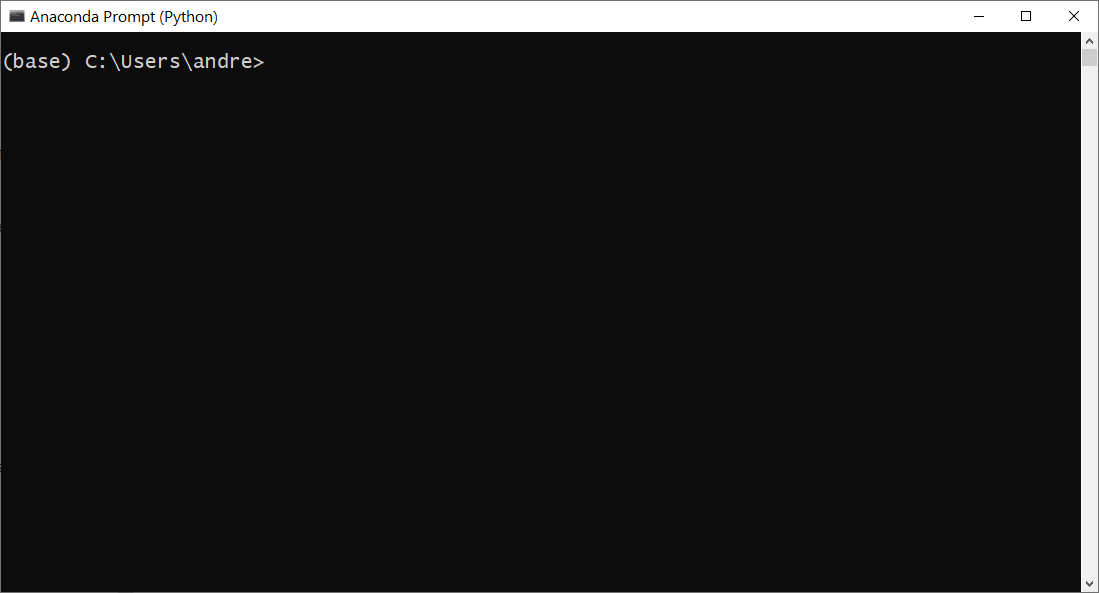
\includegraphics{screenshots/Ch01_00.PNG}

Adelante, escribe \texttt{python\ -\/-version} en la línea de comandos,
presiona Enter y observa el resultado. Esto te dirá si has instalado
Python correctamente. Mi versión de Python es \texttt{3.8.5}. Tu versión
puede ser diferente de la que utilicé para escribir este libro, pero
para el contenido que abordaré en este libro no supondrá ninguna
diferencia.

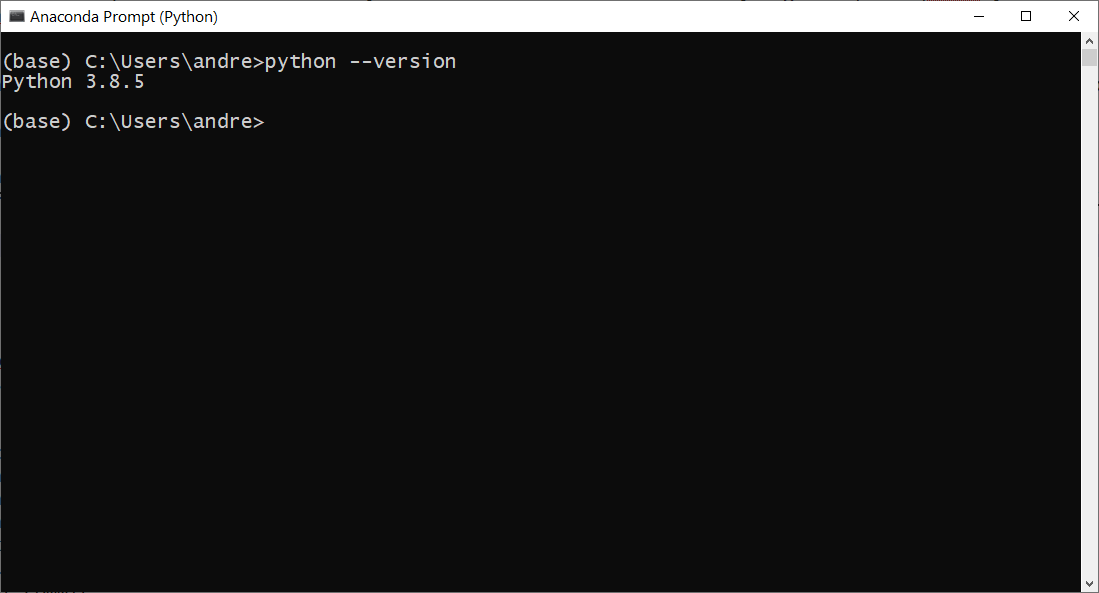
\includegraphics{screenshots/Ch01_01.PNG}

\section{Ejecución en el REPL}\label{ejecuciuxf3n-en-el-repl}

Ahora vamos a ejecutar una sesión interactiva de Python; a veces la
gente la llama el \emph{REPL}, bucle leer-evaluar-imprimir. Simplemente
escribe \texttt{python} en el símbolo del sistema y presiona Enter.
Entonces verás esta pantalla y estarás dentro de una sesión de Python.

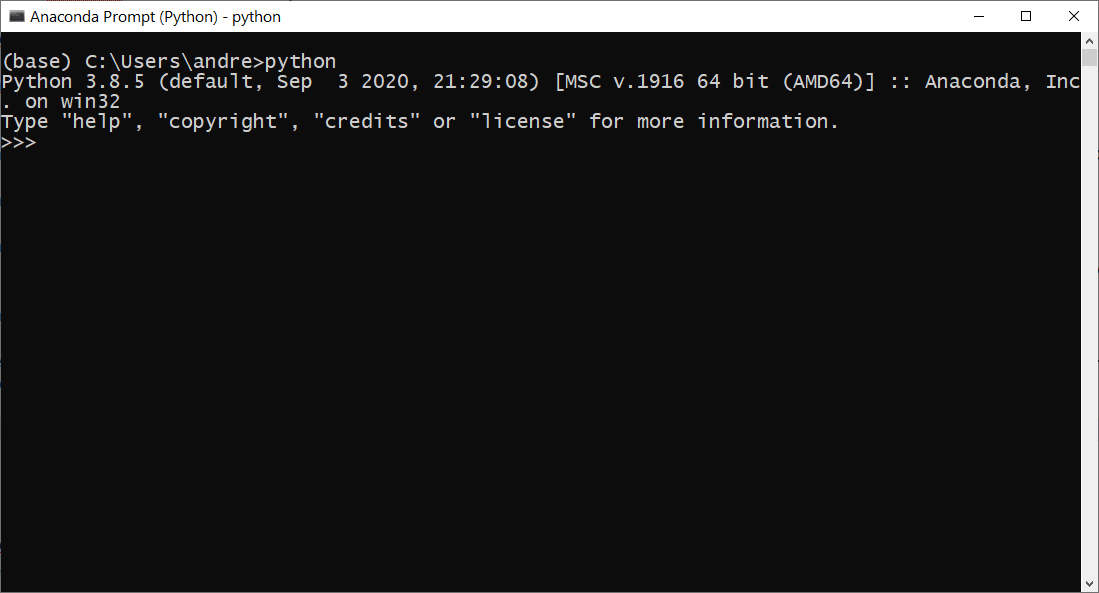
\includegraphics{screenshots/Ch01_02.PNG}

El cursor en la terminal debería estar ubicado en la parte
\texttt{\textgreater{}\textgreater{}\textgreater{}} de la pantalla.
Ahora, en el prompt, simplemente escribe \texttt{1\ +\ 2}, presiona
Enter y mostrará la respuesta:

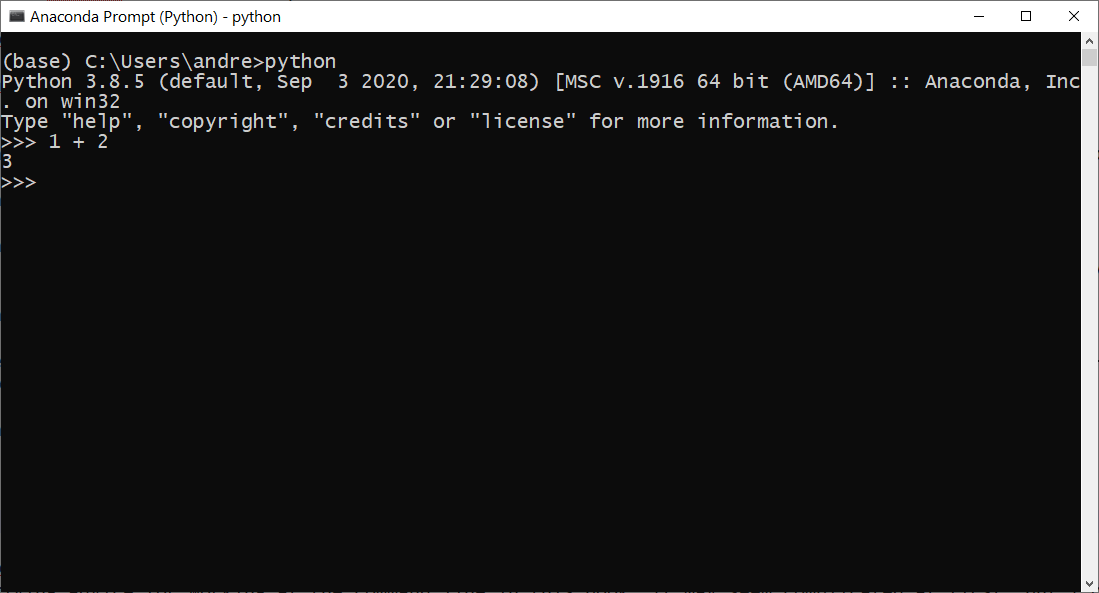
\includegraphics{screenshots/Ch01_03.PNG}

Felicidades, ahora has escrito código en Python.

\begin{tcolorbox}[enhanced jigsaw, colbacktitle=quarto-callout-note-color!10!white, arc=.35mm, opacityback=0, colframe=quarto-callout-note-color-frame, colback=white, left=2mm, leftrule=.75mm, title={Note}, bottomtitle=1mm, rightrule=.15mm, toptitle=1mm, coltitle=black, titlerule=0mm, toprule=.15mm, bottomrule=.15mm, opacitybacktitle=0.6, breakable]

Observe que la ubicación del cursor en la terminal en este punto debería
estar en la línea \texttt{\textgreater{}\textgreater{}\textgreater{}}.
No puede subir a una línea anterior en la terminal, como puede hacerlo
en un editor de texto, pero sí puede editar elementos en una sola línea
en la terminal. Así que puede escribir \texttt{1\ +\ 2} y, antes de
pulsar Enter, presione la tecla de retroceso y edite la línea para que
sea \texttt{1\ +\ 3}.

\end{tcolorbox}

\section{Ejecutar un script de
Python}\label{ejecutar-un-script-de-python}

Ahora hagamos un script de Python sencillo y llamemos a ese script desde
la línea de comandos. Primero, navega a cualquier carpeta de tu equipo
en la que puedas añadir un archivo (consulta la nota de abajo para
navegar a diferentes ubicaciones mediante la línea de comandos). Aquí
navegué a la carpeta en mi equipo
\texttt{B:\textbackslash{}code\_examples}, pero la ubicación de tu
carpeta probablemente será diferente. Crea un archivo simple, llámalo
\texttt{hello.py}, en esa misma carpeta (puedes inicializar el archivo
simplemente escribiendo \texttt{echo\ ""\ \textgreater{}\ hello.py} en
el símbolo del sistema, o \texttt{touch\ hello.py} es más fácil si estás
en una máquina Mac/Unix. O en el sistema operativo Windows crea un
archivo de texto y luego cambia la extensión a \texttt{.py} en lugar de
\texttt{.txt}).

\begin{tcolorbox}[enhanced jigsaw, colbacktitle=quarto-callout-note-color!10!white, arc=.35mm, opacityback=0, colframe=quarto-callout-note-color-frame, colback=white, left=2mm, leftrule=.75mm, title={Note}, bottomtitle=1mm, rightrule=.15mm, toptitle=1mm, coltitle=black, titlerule=0mm, toprule=.15mm, bottomrule=.15mm, opacitybacktitle=0.6, breakable]

Daré consejos para trabajar en la línea de comandos en este libro. Puede
parecer complicado al principio, pero solo tengo memorizados unos pocos
comandos. Para la gestión de proyectos, es importante saber exactamente
\emph{dónde} ejecutas los comandos. Aquí hay algunas notas sobre el uso
de \texttt{cd} para navegar a diferentes directorios:

\begin{itemize}
\tightlist
\item
  usa \texttt{cd\ YourPath\textbackslash{}YourFolder} para moverte a
  diferentes carpetas, p.~ej., en Windows podría ser
  \texttt{cd\ D:\textbackslash{}Dropbox\textbackslash{}Project},
  mientras que en Unix podría ser \texttt{cd\ /Project/sub\_folder}. En
  Windows, para cambiar a una unidad diferente, puedes simplemente
  escribir esa letra de unidad (sin \texttt{cd} al principio; p.~ej., si
  solo escribes \texttt{D:}, el símbolo del sistema cambiará el
  directorio a la unidad \texttt{D:}).
\item
  Si tu ruta tiene un espacio, debe ir entre comillas al usar
  \texttt{cd}, por ejemplo
  \texttt{cd\ "C:\textbackslash{}OneDrive\textbackslash{}OneDrive\ -\ Uni\textbackslash{}Folder"}.
  Sin las comillas, el comando \texttt{cd} dará un error.
\item
  usa \texttt{cd\ ..\textbackslash{}} (o \texttt{cd\ ../} en Unix/Mac)
  para subir una carpeta; p.~ej., si estás en
  \texttt{D:\textbackslash{}Project\textbackslash{}sub\_project} y
  escribes \texttt{cd\ ../}, ahora estarás en
  \texttt{D:\textbackslash{}Project}.
\item
  No necesitas escribir la ruta completa para bajar a una sola carpeta,
  así que si estás en \texttt{D:\textbackslash{}Project} y escribes
  \texttt{cd\ .\textbackslash{}sub\_project} bajarás al directorio
  \texttt{D:\textbackslash{}Project\textbackslash{}sub\_project}.
\item
  usa el comando \texttt{pwd} para mostrar el directorio actual.
\end{itemize}

\end{tcolorbox}

En ese archivo \texttt{hello.py} (que es solo un archivo de texto),
ábrelo con el editor de texto que prefieras. Luego escribe estas líneas
de código en ese archivo y guarda el archivo:

\begin{Shaded}
\begin{Highlighting}[]
\CommentTok{\# This is a comment line}
\NormalTok{x }\OperatorTok{=} \StringTok{\textquotesingle{}hello world\textquotesingle{}}
\BuiltInTok{print}\NormalTok{(x)}

\NormalTok{y }\OperatorTok{=} \DecValTok{3}\OperatorTok{/}\DecValTok{2}
\BuiltInTok{print}\NormalTok{(y)}
\end{Highlighting}
\end{Shaded}

Ahora, de vuelta en el símbolo del sistema, escribe
\texttt{python\ hello.py} y presiona Enter. Deberías ver que se ejecutó
tu archivo de Python y que se imprimieron los resultados.

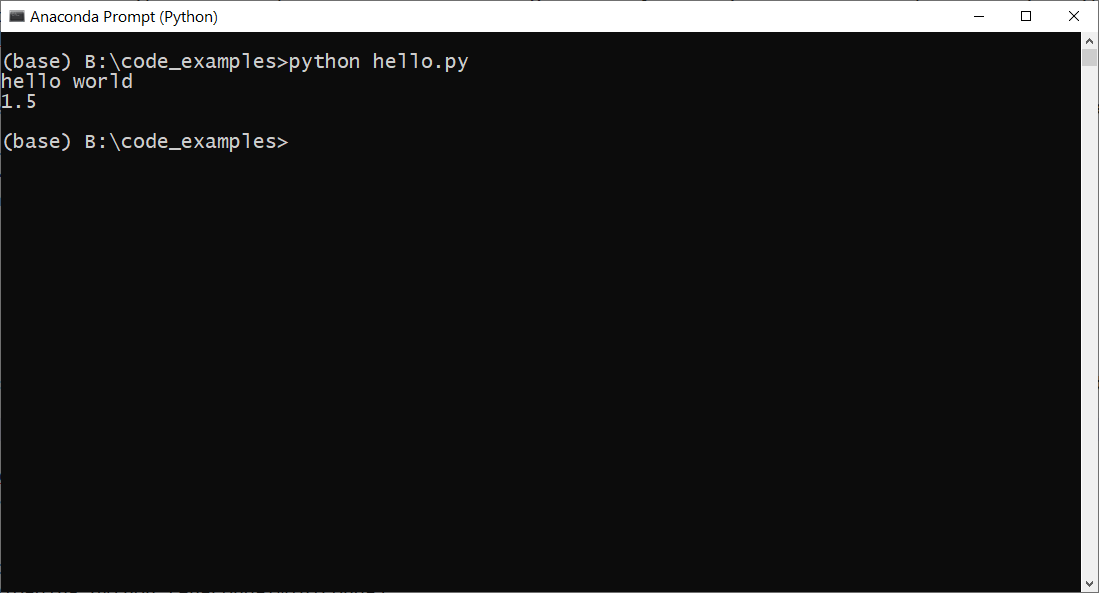
\includegraphics{screenshots/Ch01_04.PNG}

Ciertos escenarios determinarán si estás escribiendo código en una
sesión interactiva de REPL o ejecutando código mediante scripts. En la
mayor parte de mi trabajo, depuro el código inicial usando el REPL y
luego guardo el código final y ejecuto todo el conjunto de
procedimientos mediante un script.

\section{Algunas notas adicionales}\label{algunas-notas-adicionales}

Uso \href{https://notepad-plus-plus.org/}{Notepad++} para escribir gran
parte de mi código. Aquí se muestra cómo se ve el bloque de código
anterior, con Notepad++ y el propio archivo:

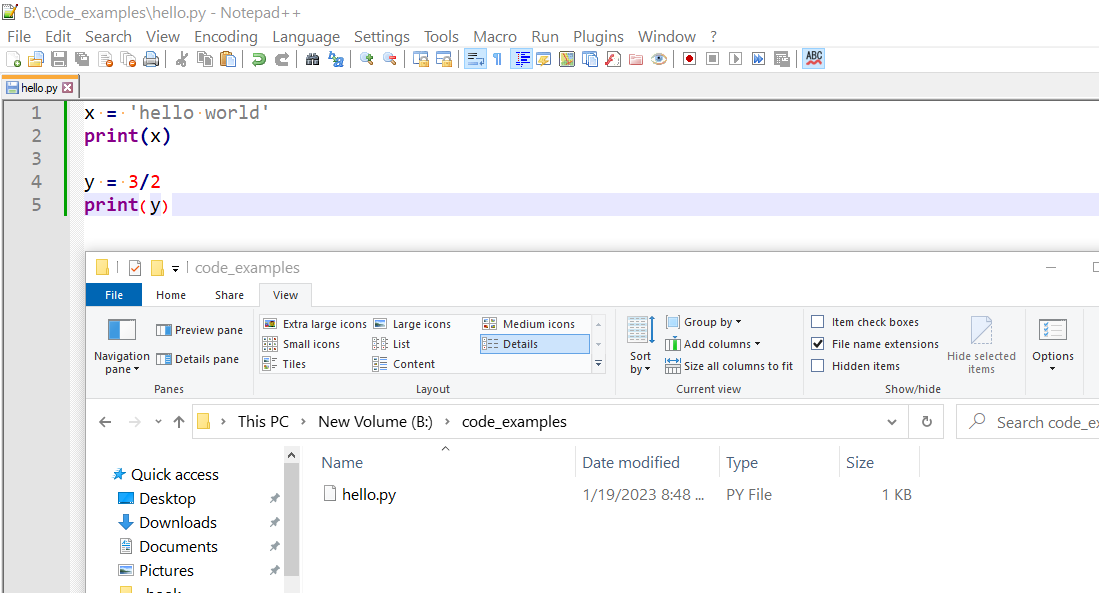
\includegraphics{screenshots/Ch01_05.PNG}

Notepad++ sabe que un archivo \texttt{.py} es un archivo de Python, y
por lo tanto ofrece un buen formato de código. También permite
configurar una opción para ver los espacios en blanco, lo cual será más
importante más adelante al escribir bloques de código condicional en
Python. (No deberías escribir código en un programa que formatea tu
texto, como Microsoft Word, ya que su autoformato puede causar errores
en tu código.)

Pero hay otras opciones que pueden ayudarte a escribir código en Python.
En ocasiones, en mi trabajo utilizo Visual Studio (VS) Code, que es todo
un IDE (entorno de desarrollo integrado). Esto solo significa que tiene
cosas adicionales (como una consola de comandos integrada y soporte para
GitHub). VS Code tiene extensiones para Python, así como para varios
otros lenguajes. Otro IDE popular para Python es PyCharm. Estos,
nuevamente, son en su mayoría intercambiables; a mí me gusta Notepad++
por su sencillez.

\begin{tcolorbox}[enhanced jigsaw, colbacktitle=quarto-callout-note-color!10!white, arc=.35mm, opacityback=0, colframe=quarto-callout-note-color-frame, colback=white, left=2mm, leftrule=.75mm, title={Note}, bottomtitle=1mm, rightrule=.15mm, toptitle=1mm, coltitle=black, titlerule=0mm, toprule=.15mm, bottomrule=.15mm, opacitybacktitle=0.6, breakable]

Aquí hay algunos comandos adicionales de la línea de comandos que uso
habitualmente:

\begin{itemize}
\tightlist
\item
  En Windows, para limpiar la terminal puedes usar \texttt{cls}; en
  Unix/Mac puedes usar \texttt{clear}
\item
  puedes usar \texttt{cat\ file.py} para mostrar en la terminal el
  contenido de un archivo
\item
  puedes usar \texttt{mkdir} para crear una nueva carpeta
\item
  puedes redirigir la salida a un archivo; p.~ej.,
  \texttt{python\ hello.py\ \textgreater{}\ log.txt} guardaría la salida
  del comando anterior en el archivo \texttt{log.txt} en lugar de
  mostrarla en la terminal.
\item
  si usas
  \texttt{python\ script.py\ \textgreater{}\textgreater{}\ log.txt},
  esto \emph{anexa} la salida al archivo de registro. Lo cual es útil
  para tareas repetitivas que se actualizan con el tiempo.
\end{itemize}

\end{tcolorbox}

Otra opción para escribir código de Python (especialmente para quienes
realizan computación científica) es usar Jupyter Notebooks. Muchos
tutoriales de Python para principiantes sugieren esto. Más adelante
incluiré un capítulo que muestra cómo crear un informe estandarizado con
Jupyter Notebooks, pero no recomiendo esta herramienta para quienes
recién comienzan. Muchos de los aspectos sobre gestión de proyectos que
trataré en este libro son difíciles de controlar con Jupyter.

Ahora que tienes los conocimientos para ejecutar código de Python, el
próximo capítulo cubrirá más conceptos básicos sobre cómo escribir
código de Python.

\bookmarksetup{startatroot}

\chapter{Primeros pasos para escribir código en
Python}\label{sec-started}

\begin{tikzpicture}[overlay, remember picture]
\node[xshift=-1.5in,yshift=-1.5in] at (current page.north east) {
\includegraphics{chap_images/C02_latex.png}};
\end{tikzpicture}

Aunque el capítulo anterior te mostró cómo ejecutar código, ya sea en el
REPL o mediante scripts, este capítulo te pondrá en marcha escribiendo
código de Python propiamente dicho. Recomiendo teclear los ejemplos de
código que aparecen en los recuadros en una sesión de REPL para
seguirlos, aunque también puedes guardarlos en scripts \texttt{.py} y
ejecutarlos directamente. Las partes en gris son lo que escribirías en
la terminal, y los recuadros azules son lo que debería imprimirse.

Este capítulo presentará una introducción al trabajo con números,
cadenas, booleanos, listas y diccionarios. Estos \emph{objetos} son los
componentes básicos de prácticamente todo el código en Python.

\begin{tcolorbox}[enhanced jigsaw, colbacktitle=quarto-callout-note-color!10!white, arc=.35mm, opacityback=0, colframe=quarto-callout-note-color-frame, colback=white, left=2mm, leftrule=.75mm, title={Note}, bottomtitle=1mm, rightrule=.15mm, toptitle=1mm, coltitle=black, titlerule=0mm, toprule=.15mm, bottomrule=.15mm, opacitybacktitle=0.6, breakable]

En una primera lectura, este capítulo (quizá todos) parecerá mucha
información y probablemente te resultará aburrido. Sugiero que lo sigas
en el REPL, pero que \emph{los leas por encima} con bastante rapidez
(especialmente los capítulos 2, 3 y 4 sobre los conceptos básicos de
objetos, cadenas y bucles). He intentado intencionalmente ser bastante
exhaustivo con lo básico. Al trabajar en proyectos reales, puede que
necesites volver a los capítulos para entender y volver a familiarizarte
con los temas. No te conviertes en experto por leer un capítulo una sola
vez, sino por escribir código repetidamente para tus propios proyectos
con el tiempo.

\end{tcolorbox}

\section{Valores numéricos}\label{valores-numuxe9ricos}

Para empezar, puedes pensar en el código de Python como \emph{objetos} y
\emph{operaciones} aplicadas a esos objetos. Por ejemplo, si ejecutas el
código de Python:

\begin{Shaded}
\begin{Highlighting}[]
\NormalTok{x }\OperatorTok{=} \DecValTok{1}
\NormalTok{y }\OperatorTok{=}\NormalTok{ x }\OperatorTok{+} \DecValTok{1}
\BuiltInTok{print}\NormalTok{(y)}
\end{Highlighting}
\end{Shaded}

\begin{verbatim}
2
\end{verbatim}

Aquí primero creamos un objeto, \texttt{x} que es \emph{asignado} un
valor de 1 mediante el símbolo \texttt{=}. Luego creamos un segundo
objeto, \texttt{y}, que es asignado el valor \texttt{x\ +\ 1}. Y
finalmente, hacemos \texttt{print} del valor del objeto \texttt{y}.
\texttt{print} es una función cuya única finalidad es mostrar el valor
(o, más específicamente, la representación en forma de cadena de ese
objeto) en la terminal (o en cualquier ubicación a la que le indiques a
python que envíe sus resultados).

\begin{tcolorbox}[enhanced jigsaw, colbacktitle=quarto-callout-note-color!10!white, arc=.35mm, opacityback=0, colframe=quarto-callout-note-color-frame, colback=white, left=2mm, leftrule=.75mm, title={Note}, bottomtitle=1mm, rightrule=.15mm, toptitle=1mm, coltitle=black, titlerule=0mm, toprule=.15mm, bottomrule=.15mm, opacitybacktitle=0.6, breakable]

En el REPL, también es posible escribir un solo elemento en una línea y
se imprimirá la salida en la terminal. Así que, en lugar de
\texttt{print(y)}, en una sesión de REPL podrías simplemente escribir
\texttt{y} y obtendrás el mismo resultado. En un script, sin embargo,
solo \texttt{print(y)} envía la salida a la terminal.

\end{tcolorbox}

En el ejemplo anterior, los objetos eran valores enteros. También puedes
tener objetos numéricos de punto flotante. Python, a diferencia de
algunos lenguajes de programación, no te obliga a definir de antemano el
tipo de objeto.

\begin{Shaded}
\begin{Highlighting}[]
\NormalTok{x }\OperatorTok{=} \OperatorTok{{-}}\DecValTok{1}
\NormalTok{y }\OperatorTok{=} \FloatTok{3.2}
\NormalTok{z }\OperatorTok{=}\NormalTok{ x}\OperatorTok{/}\NormalTok{y}
\BuiltInTok{print}\NormalTok{(z)}
\end{Highlighting}
\end{Shaded}

\begin{verbatim}
-0.3125
\end{verbatim}

Cuando se trabaja con valores numéricos, Python es inteligente y
convierte \texttt{z} aquí en un valor de tipo float, aunque use un
entero como entrada (incluso con dos enteros, p.~ej.,
\texttt{z\ =\ 1/2}, en Python \texttt{z} será un float). Puedes ver que
aquí hice una división; la mayoría de las operaciones matemáticas son
similares a lo que escribirías en cualquier calculadora, con la
excepción de que las potencias usan \texttt{**} en lugar de
\texttt{\^{}}:

\begin{Shaded}
\begin{Highlighting}[]
\CommentTok{\# Showing off the different}
\CommentTok{\# math operations}
\NormalTok{x }\OperatorTok{=} \DecValTok{2}
\BuiltInTok{print}\NormalTok{(x }\OperatorTok{{-}} \DecValTok{1}\NormalTok{)}
\BuiltInTok{print}\NormalTok{(x }\OperatorTok{+} \DecValTok{1}\NormalTok{)}
\BuiltInTok{print}\NormalTok{(x}\OperatorTok{/}\DecValTok{2}\NormalTok{)}
\BuiltInTok{print}\NormalTok{(x}\OperatorTok{*}\DecValTok{2}\NormalTok{)}
\BuiltInTok{print}\NormalTok{(x}\OperatorTok{**}\DecValTok{3}\NormalTok{)      }\CommentTok{\# x to the third power}
\BuiltInTok{print}\NormalTok{(x}\OperatorTok{**}\NormalTok{(}\DecValTok{1}\OperatorTok{/}\DecValTok{2}\NormalTok{))  }\CommentTok{\# x to the 1/2 power (square root)}
\end{Highlighting}
\end{Shaded}

\begin{verbatim}
1
3
1.0
4
8
1.4142135623730951
\end{verbatim}

Uno de los operadores especiales en Python sirve para modificar el valor
numérico de un objeto. Por ejemplo, para incrementar el valor de un
objeto en uno, podrías hacer:

\begin{Shaded}
\begin{Highlighting}[]
\NormalTok{x }\OperatorTok{=} \DecValTok{1}
\NormalTok{x }\OperatorTok{=}\NormalTok{ x }\OperatorTok{+} \DecValTok{1}
\BuiltInTok{print}\NormalTok{(x)}
\end{Highlighting}
\end{Shaded}

\begin{verbatim}
2
\end{verbatim}

Pero es más fácil usar la notación especial de \texttt{x\ +=\ 1}:

\begin{Shaded}
\begin{Highlighting}[]
\NormalTok{x }\OperatorTok{=} \DecValTok{1}
\NormalTok{x }\OperatorTok{+=} \DecValTok{1}
\BuiltInTok{print}\NormalTok{(x)}
\end{Highlighting}
\end{Shaded}

\begin{verbatim}
2
\end{verbatim}

Ten en cuenta que también puedes realizar otras operaciones matemáticas,
como restar \texttt{x\ -=\ 1}, multiplicar \texttt{x\ *=\ 2}, dividir
\texttt{x\ /=\ 2} o elevar a una potencia \texttt{x\ **=\ 2}.

Los últimos ejemplos numéricos básicos que se deben presentar son
\texttt{//}, la división entera, y \texttt{\%}, el operador de módulo.
La división entera solo devuelve los números enteros en un problema de
división, y el módulo es el resto del problema de división.

\begin{Shaded}
\begin{Highlighting}[]
\NormalTok{x }\OperatorTok{=} \DecValTok{5}
\BuiltInTok{print}\NormalTok{(x}\OperatorTok{//}\DecValTok{2}\NormalTok{)}
\BuiltInTok{print}\NormalTok{(x }\OperatorTok{\%} \DecValTok{2}\NormalTok{)}
\end{Highlighting}
\end{Shaded}

\begin{verbatim}
2
1
\end{verbatim}

En capítulos posteriores en los que se analizan bibliotecas destinadas a
trabajar con datos tabulares (numpy y pandas), abordaré el procesamiento
de datos numéricos con mayor detalle. Como a menudo no se desea hacer
cálculos sobre un solo objeto, sino sobre un vector de múltiples
objetos.

\section{Cadenas}\label{subsec-strings}

Otro objeto básico que usarás a menudo en Python son las cadenas de
caracteres. Si encierras un conjunto de caracteres entre comillas, eso
da como resultado un objeto cadena. Aquí incluso realizo la suma de
objetos cadena, lo que concatena las dos cadenas.

\begin{Shaded}
\begin{Highlighting}[]
\NormalTok{x }\OperatorTok{=} \StringTok{"ABC"}
\NormalTok{y }\OperatorTok{=} \StringTok{"de"}
\NormalTok{z }\OperatorTok{=}\NormalTok{ x }\OperatorTok{+}\NormalTok{ y}
\BuiltInTok{print}\NormalTok{(z)}
\end{Highlighting}
\end{Shaded}

\begin{verbatim}
ABCde
\end{verbatim}

Las cadenas pueden contener cualquier carácter alfanumérico, por lo que
pueden albergar representaciones textuales de números. Ten en cuenta que
sumar dos cadenas no es lo mismo que sumar dos valores numéricos:
¡concatena las dos cadenas!

\begin{Shaded}
\begin{Highlighting}[]
\NormalTok{x }\OperatorTok{=} \StringTok{"1"}
\NormalTok{y }\OperatorTok{=} \StringTok{"3"}
\NormalTok{z }\OperatorTok{=}\NormalTok{ x }\OperatorTok{+}\NormalTok{ y}
\BuiltInTok{print}\NormalTok{(z)}
\end{Highlighting}
\end{Shaded}

\begin{verbatim}
13
\end{verbatim}

Puedes convertir cadenas a valores numéricos mediante las funciones
\texttt{int} y \texttt{float}.

\begin{Shaded}
\begin{Highlighting}[]
\NormalTok{x }\OperatorTok{=} \StringTok{"1"}
\NormalTok{xi }\OperatorTok{=} \BuiltInTok{int}\NormalTok{(x)}
\NormalTok{xf }\OperatorTok{=} \BuiltInTok{float}\NormalTok{(x)}
\BuiltInTok{print}\NormalTok{(xi,}\StringTok{","}\NormalTok{,xf) }\CommentTok{\# can print multiple objects at once}
\end{Highlighting}
\end{Shaded}

\begin{verbatim}
1 , 1.0
\end{verbatim}

Y, viceversa, puedes convertir valores numéricos en cadenas mediante la
función \texttt{str}.

\begin{Shaded}
\begin{Highlighting}[]
\NormalTok{xi }\OperatorTok{=} \DecValTok{1}
\NormalTok{xf }\OperatorTok{=} \FloatTok{1.0} \CommentTok{\# if you use decimal, will be float}

\NormalTok{xsi }\OperatorTok{=} \BuiltInTok{str}\NormalTok{(xi)}
\NormalTok{xsf }\OperatorTok{=} \BuiltInTok{str}\NormalTok{(xf)}

\BuiltInTok{print}\NormalTok{(xsi }\OperatorTok{+} \StringTok{"|"} \OperatorTok{+}\NormalTok{ xsf) }\CommentTok{\#concat the strings}
\end{Highlighting}
\end{Shaded}

\begin{verbatim}
1|1.0
\end{verbatim}

\begin{tcolorbox}[enhanced jigsaw, colbacktitle=quarto-callout-note-color!10!white, arc=.35mm, opacityback=0, colframe=quarto-callout-note-color-frame, colback=white, left=2mm, leftrule=.75mm, title={Note}, bottomtitle=1mm, rightrule=.15mm, toptitle=1mm, coltitle=black, titlerule=0mm, toprule=.15mm, bottomrule=.15mm, opacitybacktitle=0.6, breakable]

He presentado tres funciones hasta ahora, \texttt{print}, \texttt{int},
\texttt{float} y \texttt{str}. Las funciones en python adoptan la forma
\texttt{function(input)}, es decir, un nombre particular seguido de dos
paréntesis.

\end{tcolorbox}

Las cadenas pueden encerrarse con comillas simples o dobles. Sin
embargo, ten en cuenta que los caracteres especiales en las cadenas
pueden causar problemas. Las barras invertidas en las variables de ruta
de Windows son un ejemplo común:

\begin{Shaded}
\begin{Highlighting}[]
\NormalTok{project\_path }\OperatorTok{=} \StringTok{"C:\textbackslash{}Project\textbackslash{}SubFolder"}
\NormalTok{project\_path }\CommentTok{\# Note no print statement}
\end{Highlighting}
\end{Shaded}

\begin{verbatim}
'C:\\Project\\SubFolder'
\end{verbatim}

\begin{tcolorbox}[enhanced jigsaw, colbacktitle=quarto-callout-note-color!10!white, arc=.35mm, opacityback=0, colframe=quarto-callout-note-color-frame, colback=white, left=2mm, leftrule=.75mm, title={Note}, bottomtitle=1mm, rightrule=.15mm, toptitle=1mm, coltitle=black, titlerule=0mm, toprule=.15mm, bottomrule=.15mm, opacitybacktitle=0.6, breakable]

Lo que se imprime en la consola no es necesariamente la misma
representación textual del objeto en sí. Por ejemplo, prueba
\texttt{x\ =\ "Line1\textbackslash{}nLine2"} y luego escribe solo
\texttt{x} en la terminal y observa qué se imprime, a diferencia de
escribir \texttt{print(x)}. En este ejemplo, print interpreta los saltos
de línea en la cadena, mientras que simplemente escribir \texttt{x} en
una sesión REPL no lo hace.

\end{tcolorbox}

¡Puedes ver que python insertó barras invertidas adicionales! Si quieres
que la cadena quede exactamente como la escribiste, puedes usar la
opción de cadena \texttt{r""}, que significa cadena \emph{real}.

\begin{Shaded}
\begin{Highlighting}[]
\NormalTok{project\_path }\OperatorTok{=} \VerbatimStringTok{r"C:\textbackslash{}NoExtra\textbackslash{}BackSlashes"}
\BuiltInTok{print}\NormalTok{(project\_path)}
\end{Highlighting}
\end{Shaded}

\begin{verbatim}
C:\NoExtra\BackSlashes
\end{verbatim}

Si quieres una cadena de varias líneas en Python, puedes usar comillas
triples. Ten en cuenta que esta cadena tiene saltos de línea en el
objeto de cadena.

\begin{Shaded}
\begin{Highlighting}[]
\NormalTok{long\_note }\OperatorTok{=} \StringTok{\textquotesingle{}\textquotesingle{}\textquotesingle{}}
\StringTok{This is a long}
\StringTok{string note}
\StringTok{over multiple lines}
\StringTok{\textquotesingle{}\textquotesingle{}\textquotesingle{}}

\BuiltInTok{print}\NormalTok{(long\_note)}
\end{Highlighting}
\end{Shaded}

\begin{verbatim}

This is a long
string note
over multiple lines
\end{verbatim}

Si tienes una cadena muy larga, como una URL, en la que no quieres
insertar saltos de línea, puedes envolver la cadena entre paréntesis. El
intérprete de Python, al final, simplemente lo convierte en una cadena:

\begin{Shaded}
\begin{Highlighting}[]
\NormalTok{long\_url }\OperatorTok{=}\NormalTok{ (}\StringTok{"Pretend I am a super "}
            \StringTok{"long url on a single line"}\NormalTok{)}

\BuiltInTok{print}\NormalTok{(long\_url)}
\end{Highlighting}
\end{Shaded}

\begin{verbatim}
Pretend I am a super long url on a single line
\end{verbatim}

Tengo todo un capítulo, el Capítulo 3, dedicado al uso más avanzado de
las cadenas de texto.

\section{Booleanos}\label{sec-bool}

Los objetos booleanos solo pueden tener dos valores, \texttt{True} o
\texttt{False}.

\begin{Shaded}
\begin{Highlighting}[]
\BuiltInTok{print}\NormalTok{(}\DecValTok{1} \OperatorTok{==} \DecValTok{1}\NormalTok{)}
\BuiltInTok{print}\NormalTok{(}\DecValTok{2} \OperatorTok{==} \DecValTok{3}\NormalTok{)}
\end{Highlighting}
\end{Shaded}

\begin{verbatim}
True
False
\end{verbatim}

Puedes ver que uso \texttt{==} para hacer una comparación de igualdad.
Recuerda que un solo \texttt{=} es para asignación. Para indicar que no
es igual, el símbolo es \texttt{!=}:

\begin{Shaded}
\begin{Highlighting}[]
\BuiltInTok{print}\NormalTok{(}\StringTok{\textquotesingle{}a\textquotesingle{}} \OperatorTok{!=} \StringTok{\textquotesingle{}a\textquotesingle{}}\NormalTok{)}
\BuiltInTok{print}\NormalTok{(}\StringTok{\textquotesingle{}b\textquotesingle{}} \OperatorTok{!=} \StringTok{\textquotesingle{}c\textquotesingle{}}\NormalTok{)}
\end{Highlighting}
\end{Shaded}

\begin{verbatim}
False
True
\end{verbatim}

Y luego también se puede usar la lógica de menor que y mayor que:

\begin{Shaded}
\begin{Highlighting}[]
\BuiltInTok{print}\NormalTok{(}\DecValTok{1} \OperatorTok{\textless{}} \DecValTok{1}\NormalTok{)}
\BuiltInTok{print}\NormalTok{(}\DecValTok{1} \OperatorTok{\textless{}=} \DecValTok{1}\NormalTok{)}
\BuiltInTok{print}\NormalTok{(}\DecValTok{2} \OperatorTok{\textgreater{}} \DecValTok{1}\NormalTok{)}
\BuiltInTok{print}\NormalTok{(}\DecValTok{2} \OperatorTok{\textgreater{}=} \DecValTok{1}\NormalTok{)}
\end{Highlighting}
\end{Shaded}

\begin{verbatim}
False
True
True
True
\end{verbatim}

Nota: también se pueden hacer comparaciones de menor que con cadenas;
por ejemplo,
\texttt{\textquotesingle{}a\textquotesingle{}\ \textless{}\ \textquotesingle{}b\textquotesingle{}}
es \texttt{True}, pero no utilizo esto muy frecuentemente. El ejemplo de
abajo muestra un caso que probablemente no era el pretendido, ya que
accidentalmente compara representaciones en cadena de números en lugar
de números directamente.

\begin{Shaded}
\begin{Highlighting}[]
\BuiltInTok{print}\NormalTok{(}\StringTok{\textquotesingle{}10\textquotesingle{}} \OperatorTok{\textless{}} \StringTok{\textquotesingle{}2\textquotesingle{}}\NormalTok{)}
\end{Highlighting}
\end{Shaded}

\begin{verbatim}
True
\end{verbatim}

A menudo se utiliza un booleano para realizar lógica condicional en
código de Python. Así puedes tener una instrucción \texttt{if} como se
muestra a continuación:

\begin{Shaded}
\begin{Highlighting}[]
\NormalTok{a }\OperatorTok{=} \DecValTok{1}

\ControlFlowTok{if}\NormalTok{ a }\OperatorTok{==} \DecValTok{1}\NormalTok{:}
  \BuiltInTok{print}\NormalTok{(a }\OperatorTok{+} \DecValTok{1}\NormalTok{)}
\end{Highlighting}
\end{Shaded}

\begin{verbatim}
2
\end{verbatim}

Una característica particular de la sintaxis de python es que el espacio
en blanco es significativo. Para indicar que la línea \texttt{print}
está dentro de la sentencia if, anteponemos varios espacios al
principio. El número de espacios no importa, aunque debe ser
consistente. (Y técnicamente también puedes usar tabulaciones en lugar
de espacios, pero lo desaconsejo encarecidamente, ya que puede hacer que
editar los archivos sea un fastidio.)

Python usa \texttt{if}, \texttt{elif}, \texttt{else} para las sentencias
condicionales. Aquí hay un ejemplo con if y else:

\begin{Shaded}
\begin{Highlighting}[]
\NormalTok{a }\OperatorTok{=} \DecValTok{1}

\ControlFlowTok{if}\NormalTok{ a }\OperatorTok{!=} \DecValTok{1}\NormalTok{:}
  \BuiltInTok{print}\NormalTok{(}\StringTok{\textquotesingle{}a does not equal 1\textquotesingle{}}\NormalTok{)}
  \BuiltInTok{print}\NormalTok{(a }\OperatorTok{+} \DecValTok{1}\NormalTok{)}
\ControlFlowTok{else}\NormalTok{:}
  \BuiltInTok{print}\NormalTok{(}\StringTok{\textquotesingle{}I am in the else part\textquotesingle{}}\NormalTok{)}
\end{Highlighting}
\end{Shaded}

\begin{verbatim}
I am in the else part
\end{verbatim}

La forma en que funcionan estas instrucciones es que se verifica si la
primera instrucción \texttt{if} es verdadera. Si esa instrucción es
verdadera, ejecuta el código anidado en la parte del if, \emph{y luego
sale del bloque de código}. Si la instrucción \texttt{if} se evalúa como
False, entonces ejecuta el bloque de la instrucción \texttt{else} para
todos los demás casos.

A veces querrás encadenar varias comprobaciones, p.~ej., ``si A, haz Y;
de lo contrario, si B, haz X''. Para hacer eso en código de Python,
usarías \texttt{if} y luego \texttt{elif}.

\begin{Shaded}
\begin{Highlighting}[]
\NormalTok{a }\OperatorTok{=} \DecValTok{1}

\ControlFlowTok{if}\NormalTok{ a }\OperatorTok{!=} \DecValTok{1}\NormalTok{:}
  \BuiltInTok{print}\NormalTok{(}\StringTok{\textquotesingle{}a does not equal 1\textquotesingle{}}\NormalTok{)}
  \BuiltInTok{print}\NormalTok{(a }\OperatorTok{+} \DecValTok{1}\NormalTok{)}
\ControlFlowTok{elif}\NormalTok{ a }\OperatorTok{==} \DecValTok{1}\NormalTok{:}
  \BuiltInTok{print}\NormalTok{(}\StringTok{\textquotesingle{}I am in the elif part\textquotesingle{}}\NormalTok{)}
\ControlFlowTok{else}\NormalTok{:}
  \BuiltInTok{print}\NormalTok{(}\StringTok{\textquotesingle{}I am in the else part\textquotesingle{}}\NormalTok{)}
\end{Highlighting}
\end{Shaded}

\begin{verbatim}
I am in the elif part
\end{verbatim}

Si un \texttt{elif} es verdadero, ejecuta ese bloque y luego sale, igual
que la instrucción \texttt{if}. Así que, en el fragmento de código
anterior, como la instrucción \texttt{elif} es verdadera, nunca llega a
la parte \texttt{else} de la lógica condicional.

No hay nada que conecte las distintas sentencias condicionales entre sí,
por lo que no es necesario que todas las secciones hagan referencia al
mismo elemento:

\begin{Shaded}
\begin{Highlighting}[]
\NormalTok{a }\OperatorTok{=} \DecValTok{1}
\NormalTok{b }\OperatorTok{=} \StringTok{\textquotesingle{}X\textquotesingle{}}

\ControlFlowTok{if}\NormalTok{ a }\OperatorTok{!=} \DecValTok{1}\NormalTok{:}
  \BuiltInTok{print}\NormalTok{(}\StringTok{\textquotesingle{}a does not equal 1\textquotesingle{}}\NormalTok{)}
\ControlFlowTok{elif}\NormalTok{ a }\OperatorTok{==} \DecValTok{2}\NormalTok{:}
  \BuiltInTok{print}\NormalTok{(}\StringTok{\textquotesingle{}a equals 2\textquotesingle{}}\NormalTok{)}
\ControlFlowTok{elif}\NormalTok{ b }\OperatorTok{==} \StringTok{\textquotesingle{}X\textquotesingle{}}\NormalTok{:}
  \BuiltInTok{print}\NormalTok{(}\StringTok{\textquotesingle{}I am in the b check elif part\textquotesingle{}}\NormalTok{)}
\ControlFlowTok{else}\NormalTok{:}
  \BuiltInTok{print}\NormalTok{(}\StringTok{\textquotesingle{}I am in the else part\textquotesingle{}}\NormalTok{)}
\end{Highlighting}
\end{Shaded}

\begin{verbatim}
I am in the b check elif part
\end{verbatim}

Y también puedes escribir lógica condicional adicional dentro de una
estructura condicional.

\begin{Shaded}
\begin{Highlighting}[]
\NormalTok{a }\OperatorTok{=} \DecValTok{1}
\NormalTok{b }\OperatorTok{=} \StringTok{\textquotesingle{}X\textquotesingle{}}

\ControlFlowTok{if}\NormalTok{ a }\OperatorTok{!=} \DecValTok{1}\NormalTok{:}
  \BuiltInTok{print}\NormalTok{(}\StringTok{\textquotesingle{}a does not equal 1\textquotesingle{}}\NormalTok{)}
  \ControlFlowTok{if}\NormalTok{ b }\OperatorTok{==} \StringTok{\textquotesingle{}X\textquotesingle{}}\NormalTok{:}
    \BuiltInTok{print}\NormalTok{(}\StringTok{\textquotesingle{}b check in first if\textquotesingle{}}\NormalTok{)}
\ControlFlowTok{else}\NormalTok{:}
  \BuiltInTok{print}\NormalTok{(}\StringTok{\textquotesingle{}I am in the else part\textquotesingle{}}\NormalTok{)}
  \ControlFlowTok{if}\NormalTok{ b }\OperatorTok{==} \StringTok{\textquotesingle{}X\textquotesingle{}}\NormalTok{:}
    \BuiltInTok{print}\NormalTok{(}\StringTok{\textquotesingle{}b check in elif\textquotesingle{}}\NormalTok{)}
\end{Highlighting}
\end{Shaded}

\begin{verbatim}
I am in the else part
b check in elif
\end{verbatim}

A veces, en una parte de la condición, no quieres hacer nada. En esos
casos, puedes usar \texttt{pass} dentro de la condición.

\begin{Shaded}
\begin{Highlighting}[]
\NormalTok{a }\OperatorTok{=} \DecValTok{1}

\ControlFlowTok{if}\NormalTok{ a }\OperatorTok{==} \DecValTok{1}\NormalTok{:}
  \ControlFlowTok{pass} \CommentTok{\# This snippet will print nothing}
\ControlFlowTok{else}\NormalTok{:}
  \BuiltInTok{print}\NormalTok{(}\StringTok{\textquotesingle{}I am in the else part\textquotesingle{}}\NormalTok{)}
\end{Highlighting}
\end{Shaded}

Normalmente se desea poner primero las condiciones más comunes en una
serie de sentencias if, y dejar las menos comunes más abajo. Así, si en
la condición más común no haces nada y solo en condiciones más raras
realizas alguna acción, esta es una manera perfectamente razonable de
escribir tus sentencias if.

Estos ejemplos comparan solo dos objetos, pero puedes combinar múltiples
sentencias condicionales usando \texttt{and} y \texttt{or}.

\begin{Shaded}
\begin{Highlighting}[]
\CommentTok{\# and example}
\NormalTok{a }\OperatorTok{=}\NormalTok{ (}\DecValTok{1} \OperatorTok{==} \DecValTok{1}\NormalTok{) }\KeywordTok{and}\NormalTok{ (}\DecValTok{2} \OperatorTok{==} \DecValTok{2}\NormalTok{)}
\BuiltInTok{print}\NormalTok{(a)}

\NormalTok{b }\OperatorTok{=}\NormalTok{ (}\DecValTok{1} \OperatorTok{==} \DecValTok{1}\NormalTok{) }\KeywordTok{and}\NormalTok{ (}\DecValTok{2} \OperatorTok{==} \DecValTok{3}\NormalTok{)}
\BuiltInTok{print}\NormalTok{(b)}

\CommentTok{\# or example}
\NormalTok{c }\OperatorTok{=}\NormalTok{ (}\DecValTok{1} \OperatorTok{==} \DecValTok{1}\NormalTok{) }\KeywordTok{or}\NormalTok{ (}\DecValTok{2} \OperatorTok{==} \DecValTok{3}\NormalTok{)}
\BuiltInTok{print}\NormalTok{(c)}
\end{Highlighting}
\end{Shaded}

\begin{verbatim}
True
False
True
\end{verbatim}

Sin embargo, hay operadores abreviados: la y comercial para \texttt{and}
y la barra vertical para \texttt{or}:

\begin{Shaded}
\begin{Highlighting}[]
\CommentTok{\# ampersand for and}
\NormalTok{a }\OperatorTok{=}\NormalTok{ (}\DecValTok{1} \OperatorTok{==} \DecValTok{1}\NormalTok{) }\OperatorTok{\&}\NormalTok{ (}\DecValTok{2} \OperatorTok{==} \DecValTok{2}\NormalTok{)}
\BuiltInTok{print}\NormalTok{(a)}

\NormalTok{b }\OperatorTok{=}\NormalTok{ (}\DecValTok{1} \OperatorTok{==} \DecValTok{1}\NormalTok{) }\OperatorTok{\&}\NormalTok{ (}\DecValTok{2} \OperatorTok{==} \DecValTok{3}\NormalTok{)}
\BuiltInTok{print}\NormalTok{(b)}

\CommentTok{\# pipe for or}
\NormalTok{c }\OperatorTok{=}\NormalTok{ (}\DecValTok{1} \OperatorTok{==} \DecValTok{1}\NormalTok{) }\OperatorTok{|}\NormalTok{ (}\DecValTok{2} \OperatorTok{==} \DecValTok{3}\NormalTok{)}
\BuiltInTok{print}\NormalTok{(c)}
\end{Highlighting}
\end{Shaded}

\begin{verbatim}
True
False
True
\end{verbatim}

Técnicamente no necesitas los paréntesis en los ejemplos anteriores,
pero a mí me resulta mucho más fácil leer el código así y mantener
juntos distintos términos:

\begin{Shaded}
\begin{Highlighting}[]
\CommentTok{\#       This is false        But this is true}
\NormalTok{a }\OperatorTok{=}\NormalTok{ ((}\DecValTok{1} \OperatorTok{==} \DecValTok{2}\NormalTok{) }\OperatorTok{\&}\NormalTok{ (}\DecValTok{2} \OperatorTok{==} \DecValTok{2}\NormalTok{)) }\OperatorTok{|}\NormalTok{ (}\DecValTok{4} \OperatorTok{==} \DecValTok{4}\NormalTok{)}
\BuiltInTok{print}\NormalTok{(a)}
\end{Highlighting}
\end{Shaded}

\begin{verbatim}
True
\end{verbatim}

Pero la mayor parte del tiempo, si es posible, simplemente lo
descompongo en código y hago que la línea final de la instrucción if sea
lo más simple posible.

\begin{Shaded}
\begin{Highlighting}[]
\NormalTok{check1 }\OperatorTok{=}\NormalTok{ (}\DecValTok{1} \OperatorTok{==} \DecValTok{2}\NormalTok{) }\OperatorTok{\&}\NormalTok{ (}\DecValTok{2} \OperatorTok{==} \DecValTok{2}\NormalTok{) }\CommentTok{\# This is false}
\NormalTok{check2 }\OperatorTok{=}\NormalTok{ (}\DecValTok{4} \OperatorTok{==} \DecValTok{4}\NormalTok{)            }\CommentTok{\# This is true}

\ControlFlowTok{if}\NormalTok{ check1 }\OperatorTok{\&}\NormalTok{ check2:}
  \BuiltInTok{print}\NormalTok{(}\StringTok{\textquotesingle{}Both check1 and check2 are true\textquotesingle{}}\NormalTok{)}
\ControlFlowTok{elif}\NormalTok{ check1 }\OperatorTok{|}\NormalTok{ check2:}
  \BuiltInTok{print}\NormalTok{(}\StringTok{\textquotesingle{}At least one of check1 or check2 are true\textquotesingle{}}\NormalTok{)}
\ControlFlowTok{else}\NormalTok{:}
  \BuiltInTok{print}\NormalTok{(}\StringTok{\textquotesingle{}Neither check1 or check2 are true\textquotesingle{}}\NormalTok{)}
\end{Highlighting}
\end{Shaded}

\begin{verbatim}
At least one of check1 or check2 are true
\end{verbatim}

En ocasiones no se utilizan los operadores matemáticos para generar las
expresiones booleanas, sino \texttt{is} o \texttt{is\ not}. Quizás el
uso más común de esto es con el objeto \texttt{None}, que puede
considerarse un valor faltante en Python.

\begin{Shaded}
\begin{Highlighting}[]
\NormalTok{x }\OperatorTok{=} \VariableTok{None}

\ControlFlowTok{if}\NormalTok{ x }\KeywordTok{is} \VariableTok{None}\NormalTok{:}
  \BuiltInTok{print}\NormalTok{(}\StringTok{\textquotesingle{}x has no value\textquotesingle{}}\NormalTok{)}
\ControlFlowTok{else}\NormalTok{:}
  \BuiltInTok{print}\NormalTok{(}\StringTok{\textquotesingle{}x has some value\textquotesingle{}}\NormalTok{)}
\end{Highlighting}
\end{Shaded}

\begin{verbatim}
x has no value
\end{verbatim}

Técnicamente, cuando escribes \texttt{a\ is\ b}, no solo verifica los
valores de los objetos, sino también que haga referencia al \emph{mismo
objeto exacto} en memoria. Técnicamente, \texttt{x\ ==\ None} funcionará
en el ejemplo anterior, pero es práctica común escribirlo de la forma
\texttt{x\ is\ None}. También puedes comprobar la condición opuesta
mediante \texttt{is\ not\ None}:

\begin{Shaded}
\begin{Highlighting}[]
\NormalTok{x }\OperatorTok{=} \VariableTok{None}

\ControlFlowTok{if}\NormalTok{ x }\KeywordTok{is} \KeywordTok{not} \VariableTok{None}\NormalTok{:}
  \BuiltInTok{print}\NormalTok{(}\StringTok{\textquotesingle{}x has some value\textquotesingle{}}\NormalTok{)}
\ControlFlowTok{else}\NormalTok{:}
  \BuiltInTok{print}\NormalTok{(}\StringTok{\textquotesingle{}x is None\textquotesingle{}}\NormalTok{)}
\end{Highlighting}
\end{Shaded}

\begin{verbatim}
x is None
\end{verbatim}

Como ejemplo final, se pueden omitir por completo los operadores de
comparación o las sentencias if. Si pasas un objeto ``vacío'' a una
sentencia if, Python comprueba si el objeto tiene algún elemento y
devuelve \texttt{True} si es así. Así que si pasas una cadena vacía, la
sentencia if devuelve \texttt{False} aquí:

\begin{Shaded}
\begin{Highlighting}[]
\NormalTok{x }\OperatorTok{=} \StringTok{\textquotesingle{}\textquotesingle{}}

\ControlFlowTok{if}\NormalTok{ x:}
  \BuiltInTok{print}\NormalTok{(}\StringTok{\textquotesingle{}x has some value\textquotesingle{}}\NormalTok{)}
\ControlFlowTok{else}\NormalTok{:}
  \BuiltInTok{print}\NormalTok{(}\StringTok{\textquotesingle{}x is an empty string\textquotesingle{}}\NormalTok{)}
\end{Highlighting}
\end{Shaded}

\begin{verbatim}
x is an empty string
\end{verbatim}

Esto funciona para otros objetos de Python, como listas y diccionarios
vacíos, lo cual se ilustrará en la sección siguiente.

\section{Listas}\label{listas}

Es importante para los principiantes comprender los diferentes objetos
que son contenedores de otros objetos. El primero es un objeto de tipo
\emph{lista}. Una lista contiene varios otros objetos, y se crea una
lista colocando elementos dentro de corchetes y separando los elementos
con comas. ¡Es más fácil mostrarlo que explicarlo con palabras!

\begin{Shaded}
\begin{Highlighting}[]
\NormalTok{x }\OperatorTok{=}\NormalTok{ [}\DecValTok{1}\NormalTok{,}\DecValTok{2}\NormalTok{,}\DecValTok{3}\NormalTok{]}
\BuiltInTok{print}\NormalTok{(x)}
\end{Highlighting}
\end{Shaded}

\begin{verbatim}
[1, 2, 3]
\end{verbatim}

Las listas pueden contener distintos tipos de objetos; por ejemplo,
pueden incluir tanto cadenas como valores numéricos en la misma lista.
Aquí también muestro que las listas pueden contener otros objetos de
Python definidos previamente.

\begin{Shaded}
\begin{Highlighting}[]
\NormalTok{a }\OperatorTok{=} \DecValTok{1}
\NormalTok{b }\OperatorTok{=} \StringTok{\textquotesingle{}z\textquotesingle{}}
\NormalTok{x }\OperatorTok{=}\NormalTok{ [a,b,}\DecValTok{3}\NormalTok{]}
\BuiltInTok{print}\NormalTok{(x)}
\end{Highlighting}
\end{Shaded}

\begin{verbatim}
[1, 'z', 3]
\end{verbatim}

Puedes dividir los elementos de una lista en varias líneas en el
intérprete de Python; detecta el corchete de cierre para saber que la
entrada de la lista ha terminado. Así que la lista resultante a
continuación es exactamente la misma que \texttt{x\ =\ {[}1,2,3{]}},
solo que es otra forma de escribirla (puede ser útil dividir listas muy
largas en varias líneas para mejorar la legibilidad de tu código).

\begin{Shaded}
\begin{Highlighting}[]
\CommentTok{\# it is ok to define lists}
\CommentTok{\# over multiple lines}
\NormalTok{x }\OperatorTok{=}\NormalTok{ [}\DecValTok{1}\NormalTok{,}
     \DecValTok{2}\NormalTok{,}
     \DecValTok{3}\NormalTok{]}

\CommentTok{\# it is the same as earlier}
\CommentTok{\# on a single line}
\BuiltInTok{print}\NormalTok{(x)}
\end{Highlighting}
\end{Shaded}

\begin{verbatim}
[1, 2, 3]
\end{verbatim}

Un error común al trabajar con listas es olvidar la coma. Con valores
numéricos, esto a menudo dará como resultado un error, pero con cadenas
a veces puede no dar lugar a un error, ya que Python simplemente
concatenará implícitamente las cadenas. Por ejemplo:

\begin{Shaded}
\begin{Highlighting}[]
\CommentTok{\# This is probably not what was intended}
\NormalTok{x }\OperatorTok{=}\NormalTok{ [}\StringTok{\textquotesingle{}a\textquotesingle{}} \StringTok{\textquotesingle{}b\textquotesingle{}}\NormalTok{, }\StringTok{\textquotesingle{}c\textquotesingle{}}\NormalTok{]}
\BuiltInTok{print}\NormalTok{(x)}
\end{Highlighting}
\end{Shaded}

\begin{verbatim}
['ab', 'c']
\end{verbatim}

Entonces, aquí se omitió la coma entre las dos primeras cadenas, por lo
que la lista resultante tiene solo dos elementos, y el primero es
\texttt{\textquotesingle{}ab\textquotesingle{}}.

\begin{tcolorbox}[enhanced jigsaw, colbacktitle=quarto-callout-note-color!10!white, arc=.35mm, opacityback=0, colframe=quarto-callout-note-color-frame, colback=white, left=2mm, leftrule=.75mm, title={Note}, bottomtitle=1mm, rightrule=.15mm, toptitle=1mm, coltitle=black, titlerule=0mm, toprule=.15mm, bottomrule=.15mm, opacitybacktitle=0.6, breakable]

Una ventaja de escribir listas en varias líneas es que puedes usar
edición en \emph{columna} en varios editores de texto. En Notepad++,
puedes mantener presionada la tecla Alt y seleccionar varias líneas para
editarlas a la vez. La mayoría de los editores de texto avanzados tienen
una función similar.

\end{tcolorbox}

Puedes acceder a elementos individuales de una lista mediante su índice.
Ten en cuenta que en Python los índices de las listas comienzan en 0, no
en 1, por lo que el primer elemento de una lista tiene índice 0, el
segundo elemento tiene índice 1, etc.

\begin{Shaded}
\begin{Highlighting}[]
\NormalTok{y }\OperatorTok{=}\NormalTok{ [}\StringTok{\textquotesingle{}a\textquotesingle{}}\NormalTok{,}\StringTok{\textquotesingle{}b\textquotesingle{}}\NormalTok{,}\StringTok{\textquotesingle{}c\textquotesingle{}}\NormalTok{]}
\BuiltInTok{print}\NormalTok{(y[}\DecValTok{0}\NormalTok{])}
\BuiltInTok{print}\NormalTok{(y[}\DecValTok{1}\NormalTok{])}
\BuiltInTok{print}\NormalTok{(y[}\DecValTok{2}\NormalTok{])}
\end{Highlighting}
\end{Shaded}

\begin{verbatim}
a
b
c
\end{verbatim}

También puedes usar índices \emph{negativos} para acceder a los
elementos en orden inverso en una lista. Así, -1 accede al último
elemento de una lista, -2 al penúltimo, etc.

\begin{Shaded}
\begin{Highlighting}[]
\NormalTok{y }\OperatorTok{=}\NormalTok{ [}\StringTok{\textquotesingle{}a\textquotesingle{}}\NormalTok{,}\StringTok{\textquotesingle{}b\textquotesingle{}}\NormalTok{,}\StringTok{\textquotesingle{}c\textquotesingle{}}\NormalTok{]}
\BuiltInTok{print}\NormalTok{(y[}\OperatorTok{{-}}\DecValTok{1}\NormalTok{])}
\BuiltInTok{print}\NormalTok{(y[}\OperatorTok{{-}}\DecValTok{2}\NormalTok{])}
\end{Highlighting}
\end{Shaded}

\begin{verbatim}
c
b
\end{verbatim}

Por último, en cuanto al acceso a varios elementos de una lista, puedes
usar la notación de corte (slice). Así, \texttt{x{[}1:3{]}} accedería al
segundo y tercer elemento de la lista (es equivalente a la notación
\texttt{{[},)} en matemáticas, por lo que el extremo izquierdo del corte
es cerrado y el extremo derecho es abierto).

\begin{Shaded}
\begin{Highlighting}[]
\NormalTok{y }\OperatorTok{=}\NormalTok{ [}\StringTok{\textquotesingle{}a\textquotesingle{}}\NormalTok{,}\StringTok{\textquotesingle{}b\textquotesingle{}}\NormalTok{,}\StringTok{\textquotesingle{}c\textquotesingle{}}\NormalTok{]}
\BuiltInTok{print}\NormalTok{(y[}\DecValTok{1}\NormalTok{:}\DecValTok{3}\NormalTok{]) }\CommentTok{\# note it returns a list!}
\end{Highlighting}
\end{Shaded}

\begin{verbatim}
['b', 'c']
\end{verbatim}

También puedes usar \texttt{x{[}1:{]}} para indicar, ``dame el segundo
elemento de la lista hasta el final'', o \texttt{x{[}:3{]}} para ``dame
los primeros 3 elementos de la lista.

Se puede crear una lista vacía simplemente asignando \texttt{{[}{]}} a
un valor. Otro truco útil que conviene conocer es que se puede hacer una
comprobación booleana para una lista vacía.

\begin{Shaded}
\begin{Highlighting}[]
\NormalTok{x }\OperatorTok{=}\NormalTok{ []}

\ControlFlowTok{if}\NormalTok{ x:}
  \BuiltInTok{print}\NormalTok{(}\StringTok{\textquotesingle{}The x list is not empty\textquotesingle{}}\NormalTok{)}
\ControlFlowTok{else}\NormalTok{:}
  \BuiltInTok{print}\NormalTok{(}\StringTok{\textquotesingle{}x is empty\textquotesingle{}}\NormalTok{)}
\end{Highlighting}
\end{Shaded}

\begin{verbatim}
x is empty
\end{verbatim}

Una lista vacía no tiene elementos, así que si intentas acceder a uno
generará un error. Como se mostró arriba, si intentas usar
\texttt{x{[}0{]}}, obtendrás el error \texttt{index\ out\ of\ range}.

Otra operación booleana sobre listas consiste en comprobar si un
elemento está contenido en esa lista.

\begin{Shaded}
\begin{Highlighting}[]
\NormalTok{x }\OperatorTok{=}\NormalTok{ [}\StringTok{\textquotesingle{}a\textquotesingle{}}\NormalTok{,}\StringTok{\textquotesingle{}b\textquotesingle{}}\NormalTok{,}\StringTok{\textquotesingle{}c\textquotesingle{}}\NormalTok{]}

\ControlFlowTok{if} \StringTok{\textquotesingle{}d\textquotesingle{}} \KeywordTok{in}\NormalTok{ x:}
  \BuiltInTok{print}\NormalTok{(}\StringTok{\textquotesingle{}The list has a d element\textquotesingle{}}\NormalTok{)}
\ControlFlowTok{elif} \StringTok{\textquotesingle{}c\textquotesingle{}} \KeywordTok{in}\NormalTok{ x:}
  \BuiltInTok{print}\NormalTok{(}\StringTok{\textquotesingle{}The list has a c element\textquotesingle{}}\NormalTok{)}
\ControlFlowTok{else}\NormalTok{:}
  \BuiltInTok{print}\NormalTok{(}\StringTok{\textquotesingle{}x has neither d or c\textquotesingle{}}\NormalTok{)}
\end{Highlighting}
\end{Shaded}

\begin{verbatim}
The list has a c element
\end{verbatim}

Un dato importante que debes conocer sobre las listas es que son
\emph{mutables}. ¿Qué significa eso exactamente? Significa que podemos
modificar el contenido de una lista. Así, por ejemplo, podemos
reemplazar un único elemento en una lista.

\begin{Shaded}
\begin{Highlighting}[]
\NormalTok{y }\OperatorTok{=}\NormalTok{ [}\StringTok{\textquotesingle{}a\textquotesingle{}}\NormalTok{,}\StringTok{\textquotesingle{}b\textquotesingle{}}\NormalTok{,}\StringTok{\textquotesingle{}c\textquotesingle{}}\NormalTok{]}
\BuiltInTok{print}\NormalTok{(y)}

\NormalTok{y[}\DecValTok{1}\NormalTok{] }\OperatorTok{=} \StringTok{\textquotesingle{}Z\textquotesingle{}}
\BuiltInTok{print}\NormalTok{(y)}
\end{Highlighting}
\end{Shaded}

\begin{verbatim}
['a', 'b', 'c']
['a', 'Z', 'c']
\end{verbatim}

Para un ejemplo más complicado, las listas pueden apuntar a otras
listas. Como las listas son mutables, puedes modificar la lista interna
aquí y la lista externa refleja este cambio.

\begin{Shaded}
\begin{Highlighting}[]
\NormalTok{x }\OperatorTok{=}\NormalTok{ [}\StringTok{\textquotesingle{}a\textquotesingle{}}\NormalTok{,}\StringTok{\textquotesingle{}b\textquotesingle{}}\NormalTok{,}\StringTok{\textquotesingle{}c\textquotesingle{}}\NormalTok{]}
\NormalTok{y }\OperatorTok{=}\NormalTok{ [}\DecValTok{1}\NormalTok{, x]}
\BuiltInTok{print}\NormalTok{(y)}

\CommentTok{\# if we alter x}
\CommentTok{\# y points to }
\CommentTok{\# the altered x list}
\NormalTok{x[}\DecValTok{1}\NormalTok{] }\OperatorTok{=} \StringTok{\textquotesingle{}Z\textquotesingle{}}
\BuiltInTok{print}\NormalTok{(y)}
\end{Highlighting}
\end{Shaded}

\begin{verbatim}
[1, ['a', 'b', 'c']]
[1, ['a', 'Z', 'c']]
\end{verbatim}

La forma de pensar en esto es que la lista \texttt{y} aquí no contiene
realmente el contenido de \texttt{x}, simplemente \emph{apunta al}
objeto \texttt{x}. Así que, si el objeto \texttt{x} cambia, apunta a ese
nuevo objeto \texttt{x}.

Esto puede parecer muy técnico, pero es una característica importante
del lenguaje de programación Python. Permite escribir muchos algoritmos
distintos de forma más sencilla cuando se pueden modificar listas en su
lugar.

Puedes concatenar dos listas sumándolas:

\begin{Shaded}
\begin{Highlighting}[]
\NormalTok{x }\OperatorTok{=}\NormalTok{ [}\StringTok{\textquotesingle{}a\textquotesingle{}}\NormalTok{,}\StringTok{\textquotesingle{}b\textquotesingle{}}\NormalTok{,}\StringTok{\textquotesingle{}c\textquotesingle{}}\NormalTok{]}
\NormalTok{y }\OperatorTok{=}\NormalTok{ [}\DecValTok{1}\NormalTok{,}\DecValTok{2}\NormalTok{]}
\NormalTok{z }\OperatorTok{=}\NormalTok{ x }\OperatorTok{+}\NormalTok{ y}
\BuiltInTok{print}\NormalTok{(z)}
\end{Highlighting}
\end{Shaded}

\begin{verbatim}
['a', 'b', 'c', 1, 2]
\end{verbatim}

También puedes crear una lista repetida mediante multiplicación:

\begin{Shaded}
\begin{Highlighting}[]
\NormalTok{x }\OperatorTok{=}\NormalTok{ [}\StringTok{\textquotesingle{}a\textquotesingle{}}\NormalTok{,}\StringTok{\textquotesingle{}b\textquotesingle{}}\NormalTok{,}\StringTok{\textquotesingle{}c\textquotesingle{}}\NormalTok{]}
\NormalTok{y }\OperatorTok{=}\NormalTok{ [}\DecValTok{1}\NormalTok{]}
\BuiltInTok{print}\NormalTok{(y}\OperatorTok{*}\DecValTok{3} \OperatorTok{+}\NormalTok{ x}\OperatorTok{*}\DecValTok{2}\NormalTok{)}
\end{Highlighting}
\end{Shaded}

\begin{verbatim}
[1, 1, 1, 'a', 'b', 'c', 'a', 'b', 'c']
\end{verbatim}

Las listas tienen varios \emph{métodos} para modificar su contenido; dos
de los más comunes son ordenar e invertir:

\begin{Shaded}
\begin{Highlighting}[]
\NormalTok{x }\OperatorTok{=}\NormalTok{ [}\DecValTok{3}\NormalTok{,}\DecValTok{1}\NormalTok{,}\DecValTok{2}\NormalTok{]}

\NormalTok{x.sort() }\CommentTok{\# sorting the list}
\BuiltInTok{print}\NormalTok{(x)}

\NormalTok{x.reverse() }\CommentTok{\# reverse ordering}
\BuiltInTok{print}\NormalTok{(x)}
\end{Highlighting}
\end{Shaded}

\begin{verbatim}
[1, 2, 3]
[3, 2, 1]
\end{verbatim}

\begin{tcolorbox}[enhanced jigsaw, colbacktitle=quarto-callout-note-color!10!white, arc=.35mm, opacityback=0, colframe=quarto-callout-note-color-frame, colback=white, left=2mm, leftrule=.75mm, title={Note}, bottomtitle=1mm, rightrule=.15mm, toptitle=1mm, coltitle=black, titlerule=0mm, toprule=.15mm, bottomrule=.15mm, opacitybacktitle=0.6, breakable]

Cuando ordenas o inviertes una lista, realiza esa operación y modifica
la lista \emph{en el lugar}. Así que el código \texttt{y\ =\ x.sort()}
probablemente sea incorrecto, ya que \texttt{x.sort()} no devuelve nada.
Por lo tanto, \texttt{y} no es igual a la lista ordenada, sino que es
\texttt{None}.

\end{tcolorbox}

Los métodos son funciones especiales que están vinculadas a objetos
específicos. Tienen la forma \texttt{object.method(input)}. Siempre
estarán separados del objeto base por un punto -- esto significa que no
puedes usar un punto en un nombre de variable. Por ejemplo, si escribes
\texttt{q.i\ =\ 1} en la terminal, mostrará un error indicando que
\texttt{q\ is\ not\ defined}. Estos métodos pueden aceptar argumentos
adicionales (son como funciones), pero estos ejemplos solo usan los
valores predeterminados. Por ejemplo, puedes ordenar en orden
descendente:

\begin{Shaded}
\begin{Highlighting}[]
\NormalTok{x }\OperatorTok{=}\NormalTok{ [}\DecValTok{3}\NormalTok{,}\DecValTok{1}\NormalTok{,}\DecValTok{2}\NormalTok{]}

\NormalTok{x.sort(reverse}\OperatorTok{=}\VariableTok{True}\NormalTok{) }\CommentTok{\# passing arg}
\BuiltInTok{print}\NormalTok{(x)}
\end{Highlighting}
\end{Shaded}

\begin{verbatim}
[3, 2, 1]
\end{verbatim}

\begin{tcolorbox}[enhanced jigsaw, colbacktitle=quarto-callout-note-color!10!white, arc=.35mm, opacityback=0, colframe=quarto-callout-note-color-frame, colback=white, left=2mm, leftrule=.75mm, title={Note}, bottomtitle=1mm, rightrule=.15mm, toptitle=1mm, coltitle=black, titlerule=0mm, toprule=.15mm, bottomrule=.15mm, opacitybacktitle=0.6, breakable]

Este es el primer ejemplo que he mostrado de una función que tiene un
argumento de \emph{palabra clave}, por lo que en lugar de
\texttt{function(input)} es \texttt{function(keyword=input)}. Las
funciones pueden tomar múltiples argumentos, como
\texttt{function(input1,input2)}. En este escenario el orden de los
argumentos importa, y puedes usar argumentos de palabra clave para
distinguir entre las entradas. Entraré en más detalles sobre esto en un
capítulo posterior sobre cómo definir tus propias funciones.

\end{tcolorbox}

También puedes agregar o eliminar elementos de listas:

\begin{Shaded}
\begin{Highlighting}[]
\NormalTok{x }\OperatorTok{=}\NormalTok{ [}\DecValTok{3}\NormalTok{,}\DecValTok{1}\NormalTok{,}\DecValTok{2}\NormalTok{]}

\NormalTok{x.append(}\StringTok{\textquotesingle{}a\textquotesingle{}}\NormalTok{) }\CommentTok{\# appending an item to end of list}
\BuiltInTok{print}\NormalTok{(x)}

\NormalTok{x.remove(}\DecValTok{1}\NormalTok{) }\CommentTok{\# removing an item}
\BuiltInTok{print}\NormalTok{(x)}
\end{Highlighting}
\end{Shaded}

\begin{verbatim}
[3, 1, 2, 'a']
[3, 2, 'a']
\end{verbatim}

Para encontrar la ubicación específica de un elemento en una lista,
puedes usar el método index:

\begin{Shaded}
\begin{Highlighting}[]
\NormalTok{x }\OperatorTok{=}\NormalTok{ [}\StringTok{\textquotesingle{}a\textquotesingle{}}\NormalTok{,}\StringTok{\textquotesingle{}b\textquotesingle{}}\NormalTok{,}\StringTok{\textquotesingle{}c\textquotesingle{}}\NormalTok{]}

\CommentTok{\# will be 1, the 2nd item in a list}
\NormalTok{bindex }\OperatorTok{=}\NormalTok{ x.index(}\StringTok{\textquotesingle{}b\textquotesingle{}}\NormalTok{)}
\BuiltInTok{print}\NormalTok{(bindex)}
\end{Highlighting}
\end{Shaded}

\begin{verbatim}
1
\end{verbatim}

Hay otros métodos de las listas que no he mostrado aquí; si ejecutas el
comando \texttt{dir} en un objeto, mostrará todos sus posibles métodos.
Te animo a experimentar por tu cuenta y ver cómo funcionan los demás
métodos, como \texttt{count} o \texttt{pop}.

\begin{Shaded}
\begin{Highlighting}[]
\NormalTok{x }\OperatorTok{=}\NormalTok{ [}\StringTok{\textquotesingle{}a\textquotesingle{}}\NormalTok{,}\StringTok{\textquotesingle{}b\textquotesingle{}}\NormalTok{,}\StringTok{\textquotesingle{}c\textquotesingle{}}\NormalTok{]}

\CommentTok{\# you can look at the methods}
\CommentTok{\# for a object using dir(object)}
\NormalTok{me }\OperatorTok{=} \BuiltInTok{dir}\NormalTok{(x)}

\CommentTok{\# there are many more! only}
\CommentTok{\# printing a few to save space}
\BuiltInTok{print}\NormalTok{(me[}\OperatorTok{{-}}\DecValTok{6}\NormalTok{:])}
\end{Highlighting}
\end{Shaded}

\begin{verbatim}
['index', 'insert', 'pop', 'remove', 'reverse', 'sort']
\end{verbatim}

A veces quieres un objeto similar a una lista, pero no quieres que sea
mutable (de modo que no puedas realizar operaciones como cambiar un solo
valor, agregar elementos o ordenar la lista). Esto puede ocurrir si
tienes un conjunto de constantes en tu script y sabes que nunca deberían
alterarse. Colocarlas en una \emph{tupla} es una forma de asegurarte de
que no se modifiquen accidentalmente. Las tuplas se ven casi igual que
una lista, pero usan paréntesis en lugar de corchetes:

\begin{Shaded}
\begin{Highlighting}[]
\NormalTok{y }\OperatorTok{=}\NormalTok{ (}\DecValTok{1}\NormalTok{,}\DecValTok{2}\NormalTok{,}\DecValTok{3}\NormalTok{)}
\NormalTok{y[}\DecValTok{1}\NormalTok{] }\OperatorTok{=} \DecValTok{5} \CommentTok{\# this will give an error}
\end{Highlighting}
\end{Shaded}

\begin{verbatim}
TypeError: 'tuple' object does not support item assignment
\end{verbatim}

Puede convertir una lista en una tupla mediante el comando
\texttt{tuple}:

\begin{Shaded}
\begin{Highlighting}[]
\NormalTok{y }\OperatorTok{=}\NormalTok{ [}\DecValTok{1}\NormalTok{,}\DecValTok{2}\NormalTok{,}\DecValTok{3}\NormalTok{]}
\NormalTok{z }\OperatorTok{=} \BuiltInTok{tuple}\NormalTok{(y)}
\NormalTok{y[}\DecValTok{1}\NormalTok{] }\OperatorTok{=} \DecValTok{5} \CommentTok{\# this is ok}
\BuiltInTok{print}\NormalTok{(y) }\CommentTok{\# can see y list is updated}
\NormalTok{z[}\DecValTok{1}\NormalTok{] }\OperatorTok{=} \DecValTok{5} \CommentTok{\# this is not, again cannot modify tuple}
\end{Highlighting}
\end{Shaded}

\begin{verbatim}
[1, 5, 3]
\end{verbatim}

\begin{verbatim}
TypeError: 'tuple' object does not support item assignment
\end{verbatim}

O, a la inversa, convierta una tupla en una lista mediante el comando
\texttt{list}:

\begin{Shaded}
\begin{Highlighting}[]
\NormalTok{z }\OperatorTok{=}\NormalTok{ (}\DecValTok{1}\NormalTok{,}\DecValTok{2}\NormalTok{,}\DecValTok{3}\NormalTok{)}
\NormalTok{y }\OperatorTok{=} \BuiltInTok{list}\NormalTok{(z)}
\NormalTok{y[}\DecValTok{1}\NormalTok{] }\OperatorTok{=} \DecValTok{5} \CommentTok{\# this is ok}
\BuiltInTok{print}\NormalTok{(y)}
\NormalTok{z[}\DecValTok{1}\NormalTok{] }\OperatorTok{=} \DecValTok{5} \CommentTok{\# this is not, again cannot modify tuple}
\end{Highlighting}
\end{Shaded}

\begin{verbatim}
[1, 5, 3]
\end{verbatim}

\begin{verbatim}
TypeError: 'tuple' object does not support item assignment
\end{verbatim}

Una última nota sobre las tuplas: puedes asignar varios objetos al mismo
tiempo. Así que puedes hacer:

\begin{Shaded}
\begin{Highlighting}[]
\NormalTok{x, y }\OperatorTok{=} \DecValTok{1}\NormalTok{, }\DecValTok{2}
\BuiltInTok{print}\NormalTok{(x,y)}
\end{Highlighting}
\end{Shaded}

\begin{verbatim}
1 2
\end{verbatim}

Esto se llama \emph{desempaquetado de tuplas}. La razón por la que se
llama así es que, cuando \emph{no} se desempaquetan los múltiples
valores separados por una coma, se devuelve una tupla.

\begin{Shaded}
\begin{Highlighting}[]
\NormalTok{t }\OperatorTok{=} \DecValTok{1}\NormalTok{, }\DecValTok{2}
\BuiltInTok{print}\NormalTok{(t)}
\end{Highlighting}
\end{Shaded}

\begin{verbatim}
(1, 2)
\end{verbatim}

Y puedes asignar más de dos valores:

\begin{Shaded}
\begin{Highlighting}[]
\NormalTok{a,b,c,d }\OperatorTok{=}\NormalTok{ (}\DecValTok{1}\NormalTok{,}\StringTok{\textquotesingle{}a\textquotesingle{}}\NormalTok{,}\DecValTok{6}\NormalTok{,}\OperatorTok{{-}}\FloatTok{1.2}\NormalTok{)}
\BuiltInTok{print}\NormalTok{(a,b,c,d)}
\end{Highlighting}
\end{Shaded}

\begin{verbatim}
1 a 6 -1.2
\end{verbatim}

Esto puede ser conveniente en varios ejemplos de bucles for (como se
muestra en el Capítulo 4), y cuando las funciones devuelven múltiples
valores (como se muestra en el Capítulo 5). Aparte de esto, sin embargo,
en mi experiencia las tuplas no se usan tan comúnmente como las listas.
Pero un ejemplo de uso que tienen se ilustra en la siguiente sección,
donde se necesita usar tuplas inmutables para diccionarios.

\section{Diccionarios}\label{diccionarios}

El segundo contenedor principal de elementos en python es un
diccionario. Así, para acceder a los elementos de una lista, basta con
un orden establecido: el primer elemento es \texttt{mylist{[}0{]}}, el
segundo elemento es \texttt{mylist{[}1{]}}, etc. A veces quieres poder
acceder a los elementos mediante nombres más simples; por ejemplo,
imagina que tuvieras una lista para contener la información de una
persona:

\begin{Shaded}
\begin{Highlighting}[]
\CommentTok{\# using a list to hold data}
\NormalTok{x }\OperatorTok{=}\NormalTok{ [}\StringTok{\textquotesingle{}Andy Wheeler\textquotesingle{}}\NormalTok{,}\StringTok{\textquotesingle{}Data Scientist\textquotesingle{}}\NormalTok{,}\StringTok{\textquotesingle{}2019\textquotesingle{}}\NormalTok{]}
\end{Highlighting}
\end{Shaded}

Para acceder al elemento nombre, necesitas saber que está en el índice
0; el elemento título está en el índice 1, etcétera. Probablemente sea
más fácil referirse a estos datos mediante un diccionario.

\begin{Shaded}
\begin{Highlighting}[]
\CommentTok{\# using a list to hold data}
\NormalTok{d }\OperatorTok{=}\NormalTok{ \{}\StringTok{\textquotesingle{}name\textquotesingle{}}\NormalTok{: }\StringTok{\textquotesingle{}Andy Wheeler\textquotesingle{}}\NormalTok{,}
     \StringTok{\textquotesingle{}title\textquotesingle{}}\NormalTok{:}\StringTok{\textquotesingle{}Data Scientist\textquotesingle{}}\NormalTok{,}
     \StringTok{\textquotesingle{}start\_year\textquotesingle{}}\NormalTok{: }\DecValTok{2019}\NormalTok{\}}

\BuiltInTok{print}\NormalTok{(d)}
\end{Highlighting}
\end{Shaded}

\begin{verbatim}
{'name': 'Andy Wheeler', 'title': 'Data Scientist', 'start_year':
2019}
\end{verbatim}

Ahora, es más fácil acceder a un elemento individual mediante
\texttt{dict{[}key{]}}, así que si solo quiero el nombre, simplemente lo
referencio explícitamente:

\begin{Shaded}
\begin{Highlighting}[]
\CommentTok{\# Grabbing the specific name element}
\BuiltInTok{print}\NormalTok{(d[}\StringTok{\textquotesingle{}name\textquotesingle{}}\NormalTok{])}
\end{Highlighting}
\end{Shaded}

\begin{verbatim}
Andy Wheeler
\end{verbatim}

La terminología para los diccionarios es que tienen \emph{claves} que
hacen referencia a \emph{valores}. Los valores pueden ser cualquier
cosa: valores numéricos, cadenas, listas, otros diccionarios, etc. Sin
embargo, las claves deben ser \emph{inmutables}, aunque los diccionarios
en sí sean mutables (por lo que no puedes usar una lista como clave,
pero sí puedes usar una tupla). Aquí podemos modificar los valores del
diccionario original \texttt{d} que creé. También puedes añadir un nuevo
elemento una vez creado el diccionario.

\begin{Shaded}
\begin{Highlighting}[]
\CommentTok{\# Modifying the start\_year element}
\NormalTok{d[}\StringTok{\textquotesingle{}start\_year\textquotesingle{}}\NormalTok{] }\OperatorTok{=} \DecValTok{2020}

\CommentTok{\# Adding in a new element tenure}
\NormalTok{d[}\StringTok{\textquotesingle{}tenure\textquotesingle{}}\NormalTok{] }\OperatorTok{=} \DecValTok{3}

\BuiltInTok{print}\NormalTok{(d[}\StringTok{\textquotesingle{}name\textquotesingle{}}\NormalTok{])}
\BuiltInTok{print}\NormalTok{(d[}\StringTok{\textquotesingle{}title\textquotesingle{}}\NormalTok{])}
\BuiltInTok{print}\NormalTok{(d[}\StringTok{\textquotesingle{}start\_year\textquotesingle{}}\NormalTok{])}
\BuiltInTok{print}\NormalTok{(d[}\StringTok{\textquotesingle{}tenure\textquotesingle{}}\NormalTok{])}
\end{Highlighting}
\end{Shaded}

\begin{verbatim}
Andy Wheeler
Data Scientist
2020
3
\end{verbatim}

La mayoría de las veces la gente usa cadenas como claves, ya que el
principal beneficio de los diccionarios frente a las listas es tener un
nombre para referirse a objetos específicos. Pero también puede ser un
número. Así que, si tuvieras identificadores numéricos en otra base de
datos que hacen referencia a ubicaciones específicas, podría tener
sentido escribir tu diccionario usando esos mismos identificadores
numéricos.

\begin{Shaded}
\begin{Highlighting}[]
\CommentTok{\# You can have numeric values}
\CommentTok{\# as a dictionary key}
\NormalTok{d }\OperatorTok{=}\NormalTok{ \{\} }\CommentTok{\# can init a dict as empty}
\NormalTok{d[}\DecValTok{101}\NormalTok{] }\OperatorTok{=}\NormalTok{ \{}\StringTok{\textquotesingle{}address\textquotesingle{}}\NormalTok{: }\StringTok{\textquotesingle{}Penny Lane\textquotesingle{}}\NormalTok{, }\StringTok{\textquotesingle{}tot\_crimes\textquotesingle{}}\NormalTok{: }\DecValTok{1}\NormalTok{\}}
\NormalTok{d[}\DecValTok{202}\NormalTok{] }\OperatorTok{=}\NormalTok{ \{}\StringTok{\textquotesingle{}address\textquotesingle{}}\NormalTok{: }\StringTok{\textquotesingle{}Outer Space\textquotesingle{}}\NormalTok{, }\StringTok{\textquotesingle{}tot\_crimes\textquotesingle{}}\NormalTok{: }\DecValTok{42}\NormalTok{\}}

\CommentTok{\# These show a dictionary inside of a dictionary}
\BuiltInTok{print}\NormalTok{(d[}\DecValTok{101}\NormalTok{])}
\BuiltInTok{print}\NormalTok{(d[}\DecValTok{202}\NormalTok{])}
\end{Highlighting}
\end{Shaded}

\begin{verbatim}
{'address': 'Penny Lane', 'tot_crimes': 1}
{'address': 'Outer Space', 'tot_crimes': 42}
\end{verbatim}

Y, al igual que las listas vacías, un diccionario vacío devolverá
\texttt{False} en una sentencia if booleana:

\begin{Shaded}
\begin{Highlighting}[]
\NormalTok{d }\OperatorTok{=}\NormalTok{ \{\} }\CommentTok{\# can init a dict as empty}

\ControlFlowTok{if}\NormalTok{ d:}
  \BuiltInTok{print}\NormalTok{(}\StringTok{\textquotesingle{}The dictionary d is not empty\textquotesingle{}}\NormalTok{)}
\ControlFlowTok{else}\NormalTok{:}
  \BuiltInTok{print}\NormalTok{(}\StringTok{\textquotesingle{}The dictionary d is empty\textquotesingle{}}\NormalTok{)}
\end{Highlighting}
\end{Shaded}

\begin{verbatim}
The dictionary d is empty
\end{verbatim}

Hay \emph{muchos} tipos de objetos más complicados en python; el primer
ejemplo del prefacio mostraba cómo trabajar con objetos \emph{datetime}.
Pero, bajo el capó, a menudo no son más que contenedores para realizar
distintas operaciones con los objetos que enumeré antes: valores
numéricos, cadenas, listas y diccionarios.


\backmatter

\end{document}
